% Final thing is style report, not article.
\documentclass[12pt,a4paper]{book}

\usepackage{algorithmic}
\usepackage{color}
\usepackage{amsmath}
\usepackage{tikz}
\usepackage{tabularx}
\usetikzlibrary{arrows,decorations.pathmorphing,backgrounds,positioning,fit,petri,automata,shapes,petri}

\pgfdeclarelayer{bg}
\pgfsetlayers{bg,main}

% MGK recommends these formatting settings:

% for hard-bound final submission, use:
\setlength{\oddsidemargin}{4.6mm}     % 30 mm left margin - 1 in
% for soft-bound version and techreport, use instead:
%\setlength{\oddsidemargin}{-0.4mm}    % 25 mm left margin - 1 in
\setlength{\evensidemargin}{\oddsidemargin}
\setlength{\topmargin}{-5.4mm}        % 20 mm top margin - 1 in
\setlength{\textwidth}{160mm}         % 20/25 mm right margin
\setlength{\textheight}{247mm}        % 20 mm bottom margin
\setlength{\headheight}{5mm}
\setlength{\headsep}{5mm}
\setlength{\parindent}{0mm}
\setlength{\parskip}{\medskipamount}
\renewcommand\baselinestretch{1.2}
\renewcommand\topfraction{.9}
\renewcommand\textfraction{.1}
\renewcommand\floatpagefraction{.8}

\author{Steven Smith}
\title{SLI: Speculative Lock Insertion}
\begin{document}

\tikzset{CfgInstr/.style={rectangle,minimum size=6mm}}
\tikzset{TrueCfgInstr/.style={rectangle,minimum size=6mm,fill=blue!50}}
\tikzset{DupeCfgInstr/.style={rectangle,minimum size=6mm,fill=blue!10}}
\tikzset{NewCfgInstr/.style={rectangle,minimum size=6mm,fill=red!50}}
\tikzset{stateSideEffect/.style={rectangle,draw}}
\tikzset{stateIf/.style={diamond,draw}}
\tikzset{stateTerminal/.style={circle,draw}}
\tikzset{flowChartState/.style={rectangle,draw}}
\tikzset{killEdge/.style={decorate,decoration={snake,segment length=1mm,post length=0.4mm}}}
\tikzset{swungEdge/.style={color=red}}
\tikzset{happensBeforeEdge/.style={dashed}}
\newcommand{\editorial}[1]{\textcolor{red}{\footnote{\textcolor{red}{#1}}}}
\newcommand{\needCite}{\editorial{need cite}}
\newcommand{\todo}[1]{\textcolor{red}{#1}}
\newcommand{\StateMachine}{finite state automaton}
\newcommand{\StateMachines}{finite state automata}
\newcommand{\CrashSummary}{crash summary}
\newcommand{\CrashSummaries}{crash summaries}

\newcommand{\concatDynTraces}{\oplus}
\newcommand{\interleaveDynTraces}{\otimes}
\newcommand{\survive}{\top}
\newcommand{\crash}{\bot}
\newcommand{\queue}[1]{\{#1\}}
\newcommand{\map}[1]{\{#1\}}
\newcommand{\mapIndex}[2]{#1[#2]}
\newcommand{\state}[1]{#1}

\maketitle

\chapter{Abstract}
Blah.

\chapter{Introduction}
\section{Motivation}
Concurrency bugs are becoming more common, don't always have source (abandonware, libraries), so need something which works on binaries

\section{Overview of approach}
\subsection{Pipeline}
Overview of the basic pipeline: find bugs with bug finding more, then instantiate them into an enforcement patch, then analyse the core dump/DRS log to better characterise the bug, and then instantiate a fix.

\subsection{Analysis technique}
Overview of basic analysis technique: building \StateMachines which approximate a fragment of the program and then doing the analysis on that.
Explain that \StateMachines are derived for some specific behaviour which is currently being investigated, and that the simplifications used depend on that.
Explain that the specification of the behaviour must be a simple boolean i.e. the interesting thing either happens or does not happen, but that's usually not an issue because the \StateMachines themselves are reasonably computationally powerful (although not Turing complete), so properties like ``X must never be greater than 5'' can be checked without needing to check properties of X.
Explain that \StateMachines are acyclic and finite, and hence executions are also finite; makes analysis much, much easier.
Explain that they can cross function boundaries and can include fragments from multiple program threads.
Explain that each \StateMachine corresponds to some possible point in the program execution (defined by a set of suffixes of stacks, such that at least one thread must match each of the suffixes), and that if you have a snapshot of the program in that state you can interpret the \StateMachine to predict whether the program is going to experience the behaviour which is being investigated.

This is probably a good place to give some examples and a very informal semantics; the full semantics will wait until later.

\section{Background}
All the bits you need to understand before reading the rest of the dissertation.
Fairly dumb summary of a little bit of related work.

\chapter{Finding bugs}
\section{Finding candidate bugs}
\subsection{Formal definition of the kind of bug which we look for}
\label{sect:finding_bugs:finding_candidate_bugs:formal_definition}
For the purposes of this section, we define a bug to be a tuple $(R, W, P)$ such that:

\begin{itemize}
\item[P valid] $P$ is a sequence of dynamic instructions which form a prefix of a possible execution of the program.
\item[R valid] $R$ is a sequence of dynamic instructions in a single thread such that $P \concatDynTraces R$, where $\concatDynTraces$ is simple concatenation, is a prefix of a possible execution of the program.
\item[W valid] Similarly, $W$ is a sequence of dynamic instructions in a single thread such that $P \concatDynTraces W$ is a prefix of a possible execution of the program.
\item[R atomic] $P \concatDynTraces R$ does not crash.
\item[W atomic] $P \concatDynTraces W \concatDynTraces R$ does not crash.
\item[W isolation] $W$ does not load from any locations which are stored to by $R$.
\item[Crash possible] $P \concatDynTraces (W \interleaveDynTraces R)$ can crash, where $\interleaveDynTraces$ is the interleaving of dynamic instruction traces.
\item[Concurrent] It is possible for the program to be in state S with one thread at the first instruction of $R$ while another thread is simultaneously at the first instruction of $W$.
\end{itemize}

We assume that programs execute an infinite sequence of no-op operations before the start of the program itself.

The intuition for this is that R is an operation which reads from some shared structure and W is an operation which updates it, and the bugs which we're looking for are those where inadequate synchronisation causes the read operation to crash.
The R atomic and W atomic rules ensure that we only need to consider concurrency-related bugs (if some behaviour is possible when the machines are run atomically then it clearly isn't a concurrency bug).
W isolation is a somewhat unfortunate property, and restricts the set of bugs which we can consider in an important way, but is necessary for the analysis to be tractable~\needCite{}.

\subsubsection{Assumptions about the program}

Big ones:

\begin{itemize}
\item
  Only need to consider two threads at a time.
  This is stronger than just assuming that each bug only involves two threads, because a third thread can sometimes make a race either possible or not possible, and that can lead to bug hiding as $N_r$ increases.
\item
  The no-mandatory-concurrency assumption.
\end{itemize}

\subsubsection{Effect of setting the $N_r$ and $N_w$}

Effect of setting $N_r$ and $N_w$: obviously setting it too small will miss bugs, but it's also possible to miss things by setting it too big.
This can happen if the program relies on a certain minimum level of concurrency for correctness, such that running two threads in isolation is guaranteed to crash but running them in parallel can allow the program to complete successfully.

\begin{figure}
\begin{tabular}{ll}
Read thread:

Load $t$ from loc1
Store $t$ to loc2
Load $t'$ from loc1
Load $t''$ from loc2
Crash if $t' == t''$

&

Write thread:

Load $t'''$ from loc1
Store $t'''$ to loc2
Store $t''' + 1$ to loc2
\end{tabular}
\label{fig:mandatory_concurrrency1}
\caption{Example of threads with mandatory concurrency.}
\end{figure}

\begin{figure}
\begin{tabular}{ll}
Read thread:

Load $t'$ from loc1
Load $t''$ from loc2
Crash if $t' == t''$

&

Write thread:

Load $t'''$ from loc1
Store $t'''$ to loc2
Store $t''' + 1$ to loc2
\end{tabular}
\label{fig:mandatory_concurrrency2}
\caption{Truncation of the example in figure~\ref{fig:mandatory_concurrency1}.}
\end{figure}

For example, consider the threads show in figure~\ref{fig:mandatory_concurrency1}.
Running the read thread atomically is guaranteed to crash, from any starting thread, and so there will be no valid bug tuples based on the complete definition of these threads.
On the other hand, if the read thread is truncated as shown in figure~\ref{fig:mandatory_concurrency2} then there may be such a tuple:

\begin{itemize}
\item The R atomic rule is satisfied provided that the initial value of loc1 is not equal to loc2.
\item The W atomic rule is satisfied by any initial state.
\item The concurrent rule is satisfied by this crashing interleaving:
  \begin{itemize}
  \item Load $t'$ from loc1
  \item Load $t'''$ from loc1
  \item Store $t'''$ to loc2
  \item Load $t''$ from loc2
  \item Crash if $t' == t''$
  \end{itemize}
\end{itemize}

Within the definition used by SLI, the larger program fragment is correct even though the smaller one is incorrect, and so using a larger window size can lead to bugs not being reported.

The fundamental problem here is one of mandatory concurrency: in the larger program, running the read thread in isolation is guaranteed to crash, but it can be ``rescued'' by being interleaved with the write thread.
The bug here is caused by insufficient concurrency, but SLI is only capable of handling bugs caused by excessive concurrency.
Excess-concurrency bugs are far more common than insufficient-concurrency bugs, for several reasons:

\begin{itemize}
\item
  An insufficient-concurrency bug indicates that the programmer got the sequential case wrong but the concurrent case correct.
  The concurrent case is usually far more difficult to design and reason about than the sequential one, and so this is an unusual outcome\needCite{}.
\item
  The sequential case generally receives more testing than the concurrent one, simply as an artifact of the way most test cases are constructed\needCite{}.
\item
  For most programs, there are far more concurrent executions than sequential ones, and so it is more likely that there are errors on an untested concurrent path than that there are errors on an untested sequential one.
\end{itemize}

SLI therefore completely ignores these insufficient-concurrency bugs.

\todo{Mention something about finding a bunch of insufficient-concurrency bugs related to malloc() failure.}

\begin{figure}
Illustration of a bug tuple.  We have a prefix P, write section W, and read section R.
\label{fig:mandatory_concurrency3}
\end{figure}

Fortunately, an insufficient-concurrency bug is the only case in which increasing the sizes of the analysis windows $N_r$ and $N_w$ can lead to bugs being masked.
To see this, consider execution shown in figure~\ref{fig:mandatory_concurrency3}.
Suppose that this execution does not generate a bug tuple.
Then moving an instruction from $R$ or $W$ into $P$ also cannot generate a bug tuple, and so by induction no smaller analysis windows can generate bug tuples.

From the fact that larger windows do not generate bug tuples, we know that:

\begin{itemize}
\item $P \concatDynTraces R \not= \survive$, from the R atomic rule, or
\item $P \concatDynTraces W \concatDynTraces R \not= \survive$, from the W atomic rule, or
\item $\crash \notin P \concatDynTraces (R \interleaveDynTraces W)$, from the concurrent rule.
\end{itemize}

Define $W = w \concatDynTraces W'$ and $R = r \concatDynTraces R'$, so that $w$ is the first instruction of $W$ and $W'$ all the others, and likewise for $r$, $R$, and $R'$.
Shrinking the analysis window then corresponds to replacing $R$ with $R'$ and $P$ with $P \concatDynTraces r$, or replacing $W$ with $W'$ and $P$ with $P \concatDynTraces w$.
We therefore generate a bug tuple with the reduced window if:

\begin{align*}
( & (P \concatDynTraces w \concatDynTraces R & = & \survive) & \wedge \\
  & (P \concatDynTraces W \concatDynTraces R & = & \survive) & \wedge \\
  & ((P \concatDynTraces w \concatDynTraces (R \interleaveDynTraces W')) & \ni & \crash)) & \vee \\
( & (P \concatDynTraces R & = & \survive) & \wedge \\
  & (P \concatDynTraces r \concatDynTraces W \concatDynTraces R' & = & \survive) & \wedge \\
  & ((P \concatDynTraces r \concatDynTraces (R' \interleaveDynTraces W)) & \ni & \crash))
\end{align*}

Combining those together, we find that reducing the analysis window can introduce a new bug if:

\begin{align*}
( & (P \concatDynTraces R & \not= & \survive) & \wedge \\
  & (P \concatDynTraces W \concatDynTraces R & \not= & \survive) & \wedge \\
  & ((P \concatDynTraces (R \interleaveDynTraces W)) & \not{}\ni & \crash)) & \vee \\
( & (P \concatDynTraces w \concatDynTraces R & = & \survive) & \wedge \\
  & (P \concatDynTraces W \concatDynTraces R & = & \survive) & \wedge \\
  & ((P \concatDynTraces w \concatDynTraces (R \interleaveDynTraces W')) & \ni & \crash)) & \vee \\
( & (P \concatDynTraces R & = & \survive) & \wedge \\
  & (P \concatDynTraces r \concatDynTraces W \concatDynTraces R' & = & \survive) & \wedge \\
  & ((P \concatDynTraces r \concatDynTraces (R' \interleaveDynTraces W)) & \ni & \crash))
\end{align*}

Simple boolean algebra, plus the obvious rule that $P \concatDynTraces (R \interleaveDynTraces W) = (P \concatDynTraces r \concatDynTraces (R' \interleaveDynTraces W) ) \cup (P \concatDynTraces w \concatDynTraces (R \interleaveDynTraces W') ) $, reduces that to this:

\begin{align*}
( & (P \concatDynTraces r \concatDynTraces R' & = & \crash) & \wedge \\
  & (P \concatDynTraces w \concatDynTraces r \concatDynTraces R' & = & \survive) & \wedge \\
  & (P \concatDynTraces w \concatDynTraces W' \concatDynTraces r \concatDynTraces R' & = & \survive) & \wedge \\
  & ((P \concatDynTraces w \concatDynTraces (W' \interleaveDynTraces R)) & \ni & \crash)) & \vee \\
( & (P \concatDynTraces r \concatDynTraces R' & = & \survive) & \wedge \\
  & (P \concatDynTraces w \concatDynTraces W' \concatDynTraces r \concatDynTraces R' & = & \crash) & \wedge \\
  & (P \concatDynTraces w \concatDynTraces r \concatDynTraces R' & = & \survive) & \wedge \\
  & (P \concatDynTraces r \concatDynTraces w \concatDynTraces W' \concatDynTraces R' & = & \survive) & \wedge \\
  & ((P \concatDynTraces r \concatDynTraces (W \interleaveDynTraces R')) & \ni & \crash))
\end{align*}

Consider the first clause of the disjunction first, and in particular consider these two terms:

\begin{align*}
 & (P \concatDynTraces r \concatDynTraces R' & = & \crash) & \wedge \\
 & (P \concatDynTraces w \concatDynTraces r \concatDynTraces R' & = & \survive)
\end{align*}

The definition of crash used in SLI is that the final instruction of $R'$ crashes, and so adding further instructions after that point cannot possible change the result.
Those terms are therefore equivalent to these:

\begin{align*}
 & (P \concatDynTraces r \concatDynTraces R' \concatDynTraces w \concatDynTraces W' & = & \crash) & \wedge \\
 & (P \concatDynTraces w \concatDynTraces r \concatDynTraces R' \concatDynTraces W' & = & \survive)
\end{align*}

In other words, $R$ is doomed when run in isolation, but running it in parallel with $W$ can save it.
That is precisely the definition of mandatory concurrency used above.

Consider the second clause now.
That contains these two terms:

\begin{align*}
  & (P \concatDynTraces w \concatDynTraces W' \concatDynTraces r \concatDynTraces R' & = & \crash) & \wedge \\
  & (P \concatDynTraces r \concatDynTraces w \concatDynTraces W' \concatDynTraces R' & = & \survive)
\end{align*}

This is even more clear: running $W$ and then $R$ atomically leads to a crash, but allowing $W$ to interrupt $R$ saves the execution.
Once again, this clause is only satisfiable in the presence of mandatory concurrency.

Therefore, it is only possible for shrinking the analysis window to reveal more bugs in the presence of mandatory concurrency, and, conversely, when the program does not use mandatory concurrency, enlarging the analysis window cannot disguise bugs.
This monotonicity property is useful because it provides a simple rule for setting the size of the analysis window: use the largest such that the analysis completes in a reasonable amount of time.
There is no need for the user to carefully select a window size for their program, or to try multiple window sizes in order to reveal additional bugs.

\todo{This proof feels quite circular and unconvincing.  May need more though here.}

\subsection{Crash summaries}

This analysis produces a series of crash summaries.
Each summary represents a (possibly infinite) set of bug tuples has several components:

\begin{itemize}
\item The read \StateMachine, corresponding to the $R$ member of the bug tuple.
\item The write \StateMachine, corresponding to the $W$ member of the bug tuple.
\item The verification condition, a predicate on the program's state which corresponds to the $S$ member of the bug tuple.
\item An aliasing table, which says which memory-accessing instructions in the read and write \StateMachines might access the same area of memory.
\end{itemize}

A crash summary represents a bug tuple $(R, W, S)$ if the summary's read \StateMachine includes the dynamic instruction trace $R$, its write \StateMachine includes the dynamic instruction trace $W$, and the verification condition is true of $S$.
The set of summaries produced by the analysis is defined to be complete if every possible bug tuple is represented by at least one crash summary, and sound if the crash summaries only represent valid bug tuples.
The analysis presented here is, in that sense, complete, subject to some caveats discussed in later sections, but not sound.

\subsection{Building read-side \StateMachines}

The aim of this phase of the algorithm is to find every fragment of the program which might act as the first ($R$) element of the bug tuple.
The simplest approach would be to simply enumerate every dynamic fragment containing $N_r$ instructions which ends in a memory-accessing instruction and convert each one independently into a \StateMachine.
While it would be effective, this would be extremely time consuming, especially for larger values of $N_r$, and would perform a large amount of redundant work.
SLI therefore uses a slightly more involved approach.

The core of the algorithm is to first select the final, crashing, instruction in the fragment, then to build up a static control-flow graph (CFG) containing every static instruction which might be part of the dynamic trace, unroll any loops in the graph until every path of length $N_r$ is represented, and then compile the resulting CFG into a \StateMachine.
This is repeated for every possible final instruction in the program.
The next few sections will describe this system in more detail.

\subsubsection{Building the static control-flow graph}
The first step of the algorithm, once a potentially-crashing instruction has been selected for investigation, is to build a static control-flow graph containing all of the instructions which might appear in the dynamic trace.
This is done by starting with a trivial CFG containing just the crashing instruction and then expanding it backwards, one instruction at a time, until every needed instruction has been discovered.

The simple case is that all of the needed instructions are contained within a single instruction.
In that case, the algorithm is as follows:

\begin{algorithmic}[1]
\STATE $depth \gets 0$
\STATE $pendingAtDepth \gets \queue{targetInstrAddress}$
\STATE $result \gets \map{}$
\WHILE{$depth < N_r$}
  \STATE $pendingAtNextDepth \gets \queue{}$
  \WHILE{$\neg{}empty(pendingAtDepth)$}
    \STATE $currentInstr \gets pop(pendingAtDepth)$
    \IF {$result \textrm{ has entry for } currentInstr$}
      \STATE \textbf{continue}
    \ENDIF
    \STATE $current \gets \text{decode instruction at } currentInstr$
    \STATE $\mapIndex{result}{currentInstr} \gets current$
    \STATE $predecessors \gets \text{predecessors of } currentInstr$
    \STATE Add $predecessors$ to $pendingAtNextDepth$
  \ENDWHILE
  \STATE $pendingAtDepth \gets pendingAtNextDepth$
  \STATE $depth \gets depth + 1$
\ENDWHILE
\end{algorithmic}

This algorithm builds, in $result$, a mapping from instruction addresses to decoded instructions, working backwards from the address of the potentially crashing instruction until every instruction which might be executed up to $N_r$ dynamic instructions before the target is present.

There is a slight subtlety on line 13, when determining the predecessors of a given instruction.
This is not always obvious, given only a binary program, for three reasons:

\begin{itemize}
\item
  The program might contain indirect branches.
  It is difficult to determine statically where these might branch to.
  A conservative approach would be to assume that they might branch anywhere, but this leads to unmanageably complex CFGs even for trivial programs.
  At the same time, ignoring them completely means that many important program paths will be missed.
\item
  The AMD64 instruction set includes variable-length instructions, and so there might be several overlapping instructions which all finish at the start of the instruction currently being investigated.
  In most programs, only one of these will ever be executed, and it is important to pick the right one.
\item
  It is not always trivial to locate all of the branch instructions in a program.
\end{itemize}

SLI solves this problem using a combination of static and dynamic analysis.
First, the dynamic analysis tracks the targets of all indirect branch and call instructions.
This makes the first problem trivial (assuming that the dynamic analysis is complete).
It also means that a simple static analysis can enumerate every instruction reachable from the program's entry point (which can itself be determined from the ELF binary's metadata), hence building up a complete CFG of the entire program.
That CFG then makes solving the second and third problems trivial.

\todo{Slight complication for async OS callbacks like signal handlers.}

\todo{There are two different CFGs here.  Should maybe do some alpha conversion to remove that ambiguity.}

\todo{Point out that the CFG can have multiple roots here.}

\subsubsection{Handling loops in the CFG}
\editorial{This is very similar to the way we handle loops in the
  write-side CFG, but more complicated and harder to explain.  That
  suggests that we should maybe explain the write-side algorithm
  first, except that the write-side CFG generation algorithm uses the
  read-side CFG as one of its inputs, which then makes that much
  harder to describe.}

There may be loops in the CFGs generated by this algorithm, but SLI requires that the \StateMachines be finite and acyclic.
These loops must therefore be eliminated in a way which is guaranteed to preserve all paths of length $N_r$.
The approach SLI takes is, in essence, to unroll the loops, duplicating instructions as necessary, until every path from a root of the CFG to the target instruction is either free from cycles or of length greater than $N_r$.

\begin{tikzpicture}
  [node distance=1 and 0.3]
  \begin{scope}
    \node (A) at (0,2) [CfgInstr] {A};
    \node (B) [CfgInstr] [below=of A] {B}; 
    \node (C) [CfgInstr] [below=of B] {C}; 
    \node (D) [CfgInstr] [below=of C] {D}; 
    \draw[->] (A) -- (B);
    \draw[->] (B) -- (C);
    \draw[->] (C) -- (D);
    \draw[->] (C.east) to [bend right=90] (B.east) node (edge1) [right] {};
    \begin{pgfonlayer}{bg}
      \node (box1) [fill=black!10,fit=(A) (B) (C) (D) (edge1)] {};
    \end{pgfonlayer}
  \end{scope}
  \begin{scope}[xshift=4cm]
    \node (A) at (0,2) [CfgInstr] {A};
    \node (B) [CfgInstr] [below=of A] {B}; 
    \node (C) [CfgInstr] [below=of B] {C}; 
    \node (D) [CfgInstr] [below=of C] {D};  
    \node (C') [CfgInstr] [right=of C] {C'};
    \draw[->] (A) -- (B);
    \draw[->] (B) -- (C);
    \draw[->] (C) -- (D);
    \draw[->] (B) to [bend right=10] (C');
    \draw[->] (C') to [bend right=10] (B);
    \begin{pgfonlayer}{bg}
      \node (box2) [fill=black!10,fit=(A) (B) (C) (D) (C')] {};
    \end{pgfonlayer}
  \end{scope}
  \begin{scope}[xshift=8cm]
    \node (A) at (0,2) [CfgInstr] {A};
    \node (B) [CfgInstr] [below=of A] {B};
    \node (B') [CfgInstr] [right=of B] {B'};
    \node (C) [CfgInstr] [below=of B] {C};
    \node (D) [CfgInstr] [below=of C] {D};
    \node (C') [CfgInstr] [right=of C] {C'};
    \draw[->] (A) -- (B);
    \draw[->] (B) -- (C);
    \draw[->] (C) -- (D);
    \draw[->] (C') -- (B);
    \draw[->] (A) -- (B');
    \draw[->] (B') to [bend right=10] (C');
    \draw[->] (C') to [bend right=10] (B');
    \begin{pgfonlayer}{bg}
      \node (box3) [fill=black!10,fit=(A) (B) (C) (D) (C') (B')] {};
    \end{pgfonlayer}
  \end{scope}
  \begin{scope}[xshift=12cm]
    \node (A) at (0,2) [CfgInstr] {A};
    \node (B) [CfgInstr] [below=of A] {B};
    \node (B') [CfgInstr] [right=of B] {B'};
    \node (C) [CfgInstr] [below=of B] {C};
    \node (C') [CfgInstr] [right=of C] {C'};
    \node (C'') [CfgInstr] [right=of C'] {C''};
    \node (D) [CfgInstr] [below=of C] {D};
    \draw[->] (A) -- (B);
    \draw[->] (B) -- (C);
    \draw[->] (C) -- (D);
    \draw[->] (C') -- (B);
    \draw[->] (A) -- (B');
    \draw[->] (B') -- (C');
    \draw[->] (C'') to [bend right=10] (B');
    \draw[->] (B') to [bend right=10] (C'');
    \begin{pgfonlayer}{bg}
      \node (box4) [fill=black!10,fit=(A) (B) (C) (D) (C') (B') (C'')] {};
    \end{pgfonlayer}
  \end{scope}
  \draw[->,thick] (box1) -- (box2) node [above,midway] {duplicate C};
  \draw[->,thick] (box2) -- (box3) node [above,midway] {duplicate B};
  \draw[->,thick] (box3) -- (box4) node [above,midway] {duplicate C'};
  \draw[->,thick] (box4) -- +(2.5,0) node [above,midway] {...};
\end{tikzpicture}

The diagram shows a CFG with four instructions, A, B, C, and D, and a loop between B and C.
This loop must be removed from the CFG whilst maintaining all paths which terminate at D and which contain $N_r$ instructions.
SLI does this by duplicating nodes in the CFG so as to unroll the loop and hence increase the distance between the loop and instruction D.
Consider the leftmost diagram first.
SLI will start at instruction D and perform a depth-first traversal backwards through the graph until it finds an edge which closes a cycle; in this case, that is the edge from C to B.
We will therefore try to break the cycle along this edge.
Note that we break on the back edge, C to B, rather than the forwards edge B to C.
To break the edge, SLI duplicates the instruction at the start of the edge and all of the edges to that instruction (in this case, duplicating C to form C' and the B to C edge to form a B to C' edge).
It then redirects the breaking edge to come from the new instruction (so the edge from C to B is replaced by an edge from C' to B).
All paths which were possible in the old graph will also be possible in the new one, if duplicated nodes are treated as semantically equivalent, and the loop is now one instruction further away from the target instruction D.

There is still a cycle in this graph, and so the process will repeat.
In this case, the first cycle encountered when performing depth-first traversal backwards from D is the B to C' edge, and so the loop will be broken on that edge by duplicating B to form B'.
As before, all of the incoming edges of the duplicated node are duplicated as well, so new edges are created from A to B' and from C' to B'.
The B to C' edge is then replaced with one from B' to C'.
Again, all paths through the graph are preserved and the cycle moved further away from D.

This algorithm can be iterated as many times as necessary until the cycle is at least $N_r$ instructions away from D.
At that point, every path of length $N_r$ traverses the cycle at most once, and so the cycle can be removed completely without changing the set of possible paths through the graph.

\begin{algorithmic}
  \WHILE {graph is not cycle-free}
     \STATE $edge \gets findEdgeToBeBroken(targetInstr, \{\})$
     \IF {$edge$ is at least $N_f$ instructions from target instruction}
        \STATE {Erase $edge$ from graph}
     \ELSE
        \STATE {$newNode \gets$ duplicate of $edge.source$}
        \FORALL {$i$ incoming edge of $edge.source$}
           \STATE {Create a new edge from $newNode$ to $i.destination$}
        \ENDFOR
        \STATE {Replace $edge$ with an edge from $newNode$ to $edge.destination$}
     \ENDIF
  \ENDWHILE
\end{algorithmic}

\begin{algorithmic}
  \STATE {findEdgeToBeBroken($node$, $path$) ->}
  \FORALL {$p$ predecessor of $node$}
     \IF {$path$ contains $p$}
         \RETURN {Success; edge from $p$ to $node$}
     \ENDIF
     \STATE $r \gets findEdgeToBeBroken(p, node::path)$
     \IF {$r$ is a success}
         \RETURN $r$
     \ENDIF
  \ENDFOR
  \RETURN {Failed; graph starting at $node$ is acyclic}
\end{algorithmic}

\todo{This really isn't very well explained.}

\todo{I think I might need a proof of correctness here.}

\subsubsection{Compiling the CFG to a \StateMachine}

The result of the previous phases is a control-flow graph containing all of the instructions which might be present in the $R$ trace of the crash tuple.
The next step is to compile this CFG into a \StateMachine.
Were it not for the transformations performed in the loop unrolling phase this would be straightforward: simply decode each instruction in isolation and convert it into an appropriate fragment of \StateMachine, and then stitch all of the fragments together again in the obvious way.
Loop unrolling introduces two major complications:

\begin{itemize}
\item
  Some edges will be erased from the CFG, so that the program can branch from instruction A to instruction B but the CFG does not allow that to happen.
  The way in which the CFG is constructed ensures that this will only happen to conditional branch instructions, and will always preserve at least one successor instruction for the branch, and so the reduced branch can be compiled to a special \state{assert} node in the \StateMachine which asserts that the program proceed to one of the remaining successor instructions.
  This means that later analysis phases will only consider the desired paths through the program\editorial{Huh?}.

  In the example, the instruction C in the original program is a conditional branch operation, and so has two successor instructions.
  Loop breaking removes the edge from C to B, and so the CFG will not match the control-flow structure of the underlying program.
  Suppose that the condition is $C_D$, so that the program moves from C to D if $C_D$ is true at C and to B otherwise.
  The \StateMachine fragment for C will then be simply an assertion that $C_D$ is true.
  Likewise, the CFG requires that C' advance to B and not to D, and so its fragment of \StateMachine will just be an assertion that $C_D$ is false.

\item
  Some additional edges will have been introduced which do not correspond to anything in the original program.
  In the example, instruction A had a single successor, B, in the original program, but has multiple successors in the unrolled CFG.
  SLI handles this case by allocating a new fresh variable and then using that to index into the available successors in the CFG.
  Since there are no constraints on the value of the new variable, later phases of the analysis will be forced to consider every possible successor, as desired.
  In effect, the new variable specifies how many times the original loop should be executed.
\end{itemize}

\todo{Effect of multiply-rooted CFGs?}

\todo{Give an example of the assertions on removed edges constraining the free variables for additional edges.}

\begin{verbatim}
l1: DEC rcx <- rcx - 1
l2: STORE $0 -> *(rcx + rdx)
l3: JMP_IF_NOT_EQ rcx, 0, l1
l4:
\end{verbatim}

Produces this CFG before unrolling:

\begin{tikzpicture}
  \node (l1) at (0,2) [CfgInstr] {l1};
  \node (l2) [CfgInstr] [below=of l1] {l2};
  \node (l3) [CfgInstr] [below=of l2] {l3};
  \node (l4) [CfgInstr] [below=of l3] {l4};
  \draw[->] (l1) -- (l2);
  \draw[->] (l2) -- (l3);
  \draw[->] (l3) -- (l4);
  \draw[->] (l3.east) to [bend right=90] (l1.east) node (edge1) [right] {};
  \begin{pgfonlayer}{bg}
    \node (box1) [fill=black!10,fit=(l1) (l2) (l3) (l4) (edge1)] {};
  \end{pgfonlayer}
\end{tikzpicture}

After unrolling, the CFG might look like this:

\begin{tikzpicture}
  \node (l1) at (0,2) [CfgInstr] {l1};
  \node (l2) [CfgInstr] [below=of l1] {l2};
  \node (l3) [CfgInstr] [below=of l2] {l3};
  \node (l4) [CfgInstr] [below=of l3] {l4};
  \draw[->] (l1) -- (l2);
  \draw[->] (l2) -- (l3);
  \draw[->] (l3) -- (l4);
  \node (l1') [CfgInstr] [right=of l1] {l1'};
  \node (l2') [CfgInstr] [right=of l2] {l2'};
  \node (l3') [CfgInstr] [right=of l3] {l3'};
  \draw[->] (l1') -- (l2');
  \draw[->] (l2') -- (l3');
  \draw[->] (l3') -- (l1);
  \node (l1'') [CfgInstr] [right=of l1'] {l1''};
  \node (l2'') [CfgInstr] [right=of l2'] {l2''};
  \node (l3'') [CfgInstr] [right=of l3'] {l3''};
  \draw[->] (l1'') -- (l2'');
  \draw[->] (l2'') -- (l3'');
  \draw[->] (l3'') -- (l1');
  \begin{pgfonlayer}{bg}
    \node (box1) [fill=black!10,fit=(l1) (l2) (l3) (l4) (l1') (l2') (l3') (l1'') (l2'') (l3'')] {};
  \end{pgfonlayer}
\end{tikzpicture}

This will produce a \StateMachine something like this:

\begin{tikzpicture}
  \node[stateSideEffect,initial] (start) {$t = \text{fresh}$};
  \node[stateIf,below=of start] (l1Guard) {If $t == 0$?};
  \node[stateIf,right=of l1Guard] (l1'Guard) {If $t == 1$?};
  \node[stateSideEffect,below=of l1Guard] (l1) {$rcx = rcx - 1$};
  \node[stateSideEffect,below=of l1] (l2) {Store $0$ to $rcx + rdx$};
  \node[stateSideEffect,below=of l2] (l3) {Assert $rcx=0$};
  \node[stateTerminal,below=of l3] (l4) {l4};
  \node[stateSideEffect,right=of l1] (l1') {$rcx = rcx - 1$};
  \node[stateSideEffect,below=of l1'] (l2') {Store $0$ to $rcx + rdx$};
  \node[stateSideEffect,below=of l2'] (l3') {Assert $\neg{} rcx=0$};
  \node[stateSideEffect,right=of l1'] (l1'') {$rcx = rcx - 1$};
  \node[stateSideEffect,below=of l1''] (l2'') {Store $0$ to $rcx + rdx$};
  \node[stateSideEffect,below=of l2''] (l3'') {Assert $\neg{} rcx=0$};
  \draw[->] (start) -- (l1Guard);
  \draw[->] (l1Guard) -- node [above] {false} (l1'Guard);
  \draw[->] (l1Guard) -- node {true} (l1);
  \draw[->] (l1) -- (l2);
  \draw[->] (l2) -- (l3);
  \draw[->] (l3) -- (l4);
  \draw[->] (l1'Guard.east) to [bend left=45] node {false} (l1'');
  \draw[->] (l1'Guard.south) -- node {true} (l1');
  \draw[->] (l1') -- (l2');
  \draw[->] (l2') -- (l3');
  \draw[->] (l3') -- (l1);
  \draw[->] (l1'') -- (l2'');
  \draw[->] (l2'') -- (l3'');
  \draw[->] (l3'') -- (l1');
\end{tikzpicture}

\subsubsection{Performing additional conditional backtracking}

\subsubsection{Cross-function behaviour}

Important complications:

\begin{itemize}
\item Sometimes end up with multiply-rooted CFGs.
\item Prefer to backtrack to head-of-function; explain what effect that has on the set of paths considered.
\item Removing cycles in a way which definitely preserves all the sufficiently-short paths.
\item What happens when you back into a function call.
\end{itemize}

\subsection{Building write-side \StateMachines}

Once SLI has obtained the read-side \StateMachine, it can analyse it to determine which loads affect the ultimate prediction, and then compare this set to the dynamic model to determine which stores might potentially influence it.
The analysis must then consider all dynamic paths of $N^w$ instructions which contain at least one of those store operations.
The basic approach here is essentially the same as that used for read-side \StateMachines: convert the set of dynamic paths into a (hopefully much smaller) set of acyclic control-flow graphs and then compile those CFGs into \StateMachines.
The details of the algorithms used are, however, slightly different.

\subsubsection{Finding relevant stores}

Simple: just rip out all the optional bits of the read machine (assertions, start and end function markers) and then simplify the result machine.
Any loads left over after that are potentially relevant.
Finding the potentially-relevant stores is then just a matter of reading them out of the dynamic profiling information.

\subsubsection{Build write-side CFGs}

The input to this phase of the analysis is a set of potentially relevant static store instructions, and the analysis must build a collection of acyclic CFGs which cover all possible paths through the program which use at least one of those static instructions and which contain at most $N_w$ instructions.
\editorial{That's not quite the problem definition I used earlier, but it's a bit easier to describe.}

One important assumption here is that the set of potentially relevant store instructions is complete, in the sense that no instruction not in that set can influence the behaviour of the load machine (this follows from the assumption that the dynamic model is itself complete).
This implies that the only parts of the dynamic write path which are actually important are the potentially relevant store instructions; everything else simply acts to constrain the behaviour of those instructions.
That in turn means that it is safe to ignore any prefix or suffix of a dynamic path which does not involve any potentially-relevant store instructions, or, to put it another way, the store CFGs only need to represent dynamic paths which start and end with potentially-relevant instructions.
This is a useful simplification.

The algorithm begins by building a partial static CFG starting at each of the potentially-relevant store instructions and covering every instruction reachable within $N_w$ instructions of that point.
As with read-side CFGs, called functions are effectively inlined into each call site, and returns from the function containing the potentially-relevant store are handled by replacing the instruction with one with a synthesised call stack and restarting.
The CFGs generated by different starting instructions will often overlap; this is handled by sharing nodes between the relevant CFGs.
The resulting CFG is then trimmed to remove any instructions which cannot reach a potentially-relevant store within $N_w$ instructions.

At this point, the CFG represents a fragment of the program and contains every instruction which might be on one of the trimmed dynamic paths which need to be represented by the output CFG, and it only remains to remove any cycles from it.
As with read-side CFGs, this is accomplished by duplicating nodes so as to unroll loops until any path which uses the loop more than once must be longer than $N_w$ instructions and can hence be discarded.
There is, however, one important difference: in the read-side CFG, we are interested in any path which terminates at a specific point, whereas in the write-side CFG we need to preserve any path which starts and ends with any member of a set of interesting instructions.
This makes it more difficult to determine when a loop has been unrolled sufficiently, as it is no longer sufficient to just check the distance to a nominated target instruction.
SLI solves this problem by labelling each node in the graph with information about where it might occur in an interesting path.
This label consists of:

\begin{itemize}
\item
  For each possibly-relevant store, the minimum distance from that store to the labelled node.
\item
  For each possible-relevant store, the minimum distance from the labelled node to that store or any of its duplicates.
\end{itemize}

We only need to consider paths of length $N_w$ or less which start with one of the potentially-relevant stores and which end with a potentially-relevant store or one of its duplicates.
Therefore, if, for any node, the minimum of the first type of label plus the minimum of the second type of label exceeds $N_w$ the node can be safely discarded.
This allows us to break cycles once they have been unrolled far enough.

\begin{algorithmic}
  \STATE {Compute initial labelling of graph}
  \FORALL {$t$ in the set of potentially-relevant stores}
    \WHILE {graph rooted at $t$ is not cycle-free}
       \STATE $edge \gets findEdgeToBeBroken(t, \{\})$
       \STATE $newLabel \gets combineLabels(\text{current label of } edge.start, \text{current label of } edge.end)$
       \IF {$min(newLabel.minFrom) + min(newLabel.minTo) > N_w$}
           \STATE {remove $edge$}
       \ELSE
           \STATE $newNode <- \text{duplicate } edge.end$
           \FORALL {Edges $e$ leaving $edge.end$}
              \STATE {Create a new edge from $newNode$ to $e.end$}
           \ENDFOR
           \STATE {Set label of $newNode$ to $newLabel$}
           \STATE {Replace $edge$ with an edge from $edge.start$ to $newNode$}
       \ENDIF
    \ENDWHILE
  \ENDFOR
\end{algorithmic}

\begin{tikzpicture}
  \node (A) at (0,2) [TrueCfgInstr] {A};
  \node (B) [CfgInstr, below=of A] {B} edge [in=30,out=-30,loop] ();
  \node (C) [TrueCfgInstr, below=of B] {C};
  \draw[->] (A) -- (B);
  \draw[->] (B) -- (C);
  \draw[->] (C) to [bend left=90] (A) node (edge1) [right,midway] {~~~~~~~~};
  \begin{pgfonlayer}{bg}
    \node(box1) [fill=black!10,fit=(A) (B) (C) (edge1)] {};
  \end{pgfonlayer}
  \draw node [right=of box1] {
    \begin{tabular}{lcccc}
      labels & min to A & min from A & min to C & min from C\\
      A & 0 & 0 & 2 & 1\\
      B & 2 & 1 & 1 & 2\\
      C & 1 & 2 & 0 & 0\\
    \end{tabular}
  };
\end{tikzpicture}

\begin{tikzpicture}
  \node (A) at (0,2) [TrueCfgInstr] {A};
  \node (B) [CfgInstr, below=of A] {B};
  \node (B1) [NewCfgInstr, right=of B] {B1};
  \node (C) [TrueCfgInstr, below=of B] {C};
  \draw[->] (A) -- (B);
  \draw[->] (B) -- (C);
  \draw[->] (B) to [bend left=10] (B1);
  \draw[->,swungEdge] (B1) to [bend left=10] (B);
  \draw[->] (B1) -- (C);
  \draw[->] (C) to [bend left=90] (A) node (edge1) [right,midway] {~~~~~~~~};
  \begin{pgfonlayer}{bg}
    \node(box1) [fill=black!10,fit=(A) (B) (B1) (C) (edge1)] {};
  \end{pgfonlayer}
  \draw node [right=of box1] {
    \begin{tabular}{lcccc}
      labels & min to A & min from A & min to C & min from C\\
      A  & 0 & 0 & 2 & 1\\
      B  & 2 & 1 & 1 & 2\\
      C  & 1 & 2 & 0 & 0\\
      B1 & 2 & 2 & 1 & 3\\
    \end{tabular}
    (dupe B)
  };
\end{tikzpicture}

\begin{tikzpicture}
  \node (A) at (0,2) [TrueCfgInstr] {A};
  \node (B) [CfgInstr, below=of A] {B};
  \node (B1) [CfgInstr, right=of B] {B1};
  \node (C) [TrueCfgInstr, below=of B] {C};
  \node (A1) [NewCfgInstr,right=of C] {A1};
  \draw[->] (A) -- (B);
  \draw[->,swungEdge] (A1) -- (B);
  \draw[->] (B) -- (C);
  \draw[->] (B) to [bend left=10] (B1);
  \draw[->] (B1) -- (C);
  \draw[->] (B1) to [bend left=10] (B);
  \draw[->] (C) -- (A1);
  \begin{pgfonlayer}{bg}
    \node(box1) [fill=black!10,fit=(A) (B) (B1) (C) (edge1)] {};
  \end{pgfonlayer}
  \draw node [right=of box1] {
    \begin{tabular}{lcccc}
      labels & min to A & min from A & min to C & min from C\\
      A  & 0 & 0 & 2 & $\infty$\\
      A1 & 0 & 3 & 2 & 1\\
      B  & 2 & 1 & 1 & 2\\
      C  & 1 & 2 & 0 & 0\\
      B1 & 2 & 2 & 1 & 3\\
    \end{tabular}
    (dupe A)
  };
\end{tikzpicture}

\begin{tikzpicture}
  \node (A) at (0,2) [TrueCfgInstr] {A};
  \node (B) [CfgInstr, below=of A] {B};
  \node (B1) [CfgInstr, right=of B] {B1};
  \node (B2) [NewCfgInstr, right=of B1] {B2};
  \node (C) [TrueCfgInstr, below=of B] {C};
  \node (A1) [DupeCfgInstr,right=of C] {A1};
  \draw[->] (A) -- (B);
  \draw[->] (A1) -- (B);
  \draw[->] (B) -- (C);
  \draw[->] (B) -- (B1);
  \draw[->,swungEdge] (B1) to [bend left=10] (B2);
  \draw[->] (B1) -- (C);
  \draw[->] (B2) to [bend left=10] (B1);
  \draw[->] (B2) -- (C);
  \draw[->] (C) -- (A1);
  \begin{pgfonlayer}{bg}
    \node(box1) [fill=black!10,fit=(A) (A1) (B) (B1) (B2) (C) (edge1)] {};
  \end{pgfonlayer}
  \draw node [right=of box1] {
    \begin{tabular}{lcccc}
      labels & min to A & min from A & min to C & min from C\\
      A  & 0 & 0 & 2 & $\infty$\\
      A1 & 0 & 3 & 2 & 1\\
      B  & 2 & 1 & 1 & 2\\
      C  & 1 & 2 & 0 & 0\\
      B1 & 2 & 2 & 1 & 3\\
      B2 & 2 & 3 & 1 & 4\\
    \end{tabular}
  };
\end{tikzpicture}

\begin{tikzpicture}
  \node (A) at (0,2) [TrueCfgInstr] {A};
  \node (B) [CfgInstr, below=of A] {B};
  \node (B1) [CfgInstr, right=of B] {B1};
  \node (B2) [CfgInstr, right=of B1] {B2};
  \node (A1) [DupeCfgInstr,right=of C] {A1};
  \node (C) [TrueCfgInstr, below=of B] {C};
  \node (B3) [NewCfgInstr, below=of A1] {B3};
  \draw[->] (A) -- (B);
  \draw[->,swungEdge] (A1) -- (B3);
  \draw[->] (B) -- (C);
  \draw[->] (B) -- (B1);
  \draw[->] (B1) to [bend left=10] (B2);
  \draw[->] (B1) -- (C);
  \draw[->] (B2) to [bend left=10] (B1);
  \draw[->] (B2) -- (C);
  \draw[->] (B3) -- (C);
  \draw[->] (B3) to [bend right=45] (B1);
  \draw[->] (C) -- (A1);
  \begin{pgfonlayer}{bg}
    \node(box1) [fill=black!10,fit=(A) (A1) (B) (B1) (B2) (B3) (C) (edge1)] {};
  \end{pgfonlayer}
  \draw node [right=of box1] {
    \begin{tabular}{lcccc}
      labels & min to A & min from A & min to C & min from C\\
      A  & 0 & 0 & 2 & $\infty$\\
      A1 & 0 & 3 & 2 & 1\\
      B  & 2 & 1 & 1 & $\infty$\\
      C  & 1 & 2 & 0 & 0\\
      B1 & 2 & 2 & 1 & 3\\
      B2 & 2 & 3 & 1 & 4\\
      B3 & 2 & 4 & 1 & 2\\
    \end{tabular}
  };
\end{tikzpicture}

\begin{tikzpicture}
  \node (A) at (0,2) [TrueCfgInstr] {A};
  \node (B) [CfgInstr, below=of A] {B};
  \node (B1) [CfgInstr, right=of B] {B1};
  \node (B2) [CfgInstr, right=of B1] {B2};
  \node (A1) [DupeCfgInstr,right=of C] {A1};
  \node (C) [TrueCfgInstr, below=of B] {C};
  \node (B3) [CfgInstr, below=of A1] {B3};
  \draw[->] (A) -- (B);
  \draw[->] (A1) -- (B3);
  \draw[->] (B) -- (C);
  \draw[->] (B) -- (B1);
  \draw[->] (B1) to [bend left=10] (B2);
  \draw[->] (B1) -- (C);
  \draw[->] (B2) to [bend left=10] (B1);
  \draw[->,killEdge] (B2) to [bend left=10] (B1);
  \draw[->] (B2) -- (C);
  \draw[->] (B3) -- (C);
  \draw[->] (B3) to [bend right=45] (B1);
  \draw[->] (C) -- (A1);
  \begin{pgfonlayer}{bg}
    \node(box1) [fill=black!10,fit=(A) (A1) (B) (B1) (B2) (B3) (C) (edge1)] {};
  \end{pgfonlayer}
  \draw node [right=of box1] {
    \begin{tabular}{lcccc}
      labels & min to A & min from A & min to C & min from C\\
      A  & 0 & 0 & 2 & $\infty$\\
      A1 & 0 & 3 & 2 & 1\\
      B  & 2 & 1 & 1 & $\infty$\\
      C  & 1 & 2 & 0 & 0\\
      B1 & 2 & 2 & 1 & 3\\
      B2 & 2 & 3 & 1 & 4\\
      New label & 2 & 4 & 1 & 5\\
    \end{tabular}
  };
\end{tikzpicture}

\begin{tikzpicture}
  \node (A) at (0,2) [TrueCfgInstr] {A};
  \node (B) [CfgInstr, below=of A] {B};
  \node (B1) [CfgInstr, right=of B] {B1};
  \node (B2) [CfgInstr, right=of B1] {B2};
  \node (A1) [DupeCfgInstr,right=of C] {A1};
  \node (C) [TrueCfgInstr, below=of B] {C};
  \node (B3) [CfgInstr, below=of A1] {B3};
  \node (C1) [NewCfgInstr, below=of B3] {C1};
  \draw[->] (A) -- (B);
  \draw[->] (A1) -- (B3);
  \draw[->] (B) -- (C);
  \draw[->] (B) -- (B1);
  \draw[->] (B1) -- (B2);
  \draw[->] (B1) -- (C);
  \draw[->] (B2) -- (C);
  \draw[->] (B3) to [bend left=45] (B1);
  \draw[->] (C) -- (A1);
  \draw[->] (C1) to [bend right=90] (A1);
  \draw[->,swungEdge] (B3) -- (C1);
  \begin{pgfonlayer}{bg}
    \node(box1) [fill=black!10,fit=(A) (A1) (B) (B1) (B2) (B3) (C) (C1) (edge1)] {};
  \end{pgfonlayer}
  \draw node [right=of box1] {
    \begin{tabular}{lcccc}
      labels & min to A & min from A & min to C & min from C\\
      A  & 0 & 0 & 2 & $\infty$\\
      A1 & 0 & 3 & 2 & 1\\
      B  & 2 & 1 & 1 & $\infty$\\
      C  & 1 & 2 & 0 & 0\\
      B1 & 2 & 2 & 1 & 3\\
      B2 & 2 & 3 & 1 & 4\\
      C3 & 1 & 4 & 0 & 3\\
    \end{tabular}
  };
\end{tikzpicture}

\begin{tikzpicture}
  \node (A) at (0,2) [TrueCfgInstr] {A};
  \node (B) [CfgInstr, below=of A] {B};
  \node (B1) [CfgInstr, right=of B] {B1};
  \node (B2) [CfgInstr, right=of B1] {B2};
  \node (A1) [DupeCfgInstr,right=of C] {A1};
  \node (C) [TrueCfgInstr, below=of B] {C};
  \node (B3) [CfgInstr, below=of A1] {B3};
  \node (C1) [DupeCfgInstr, below=of B3] {C1};
  \node (B4) [NewCfgInstr, right=of B3] {B4};
  \draw[->] (A) -- (B);
  \draw[->] (A1) -- (B3);
  \draw[->] (B) -- (C);
  \draw[->] (B) -- (B1);
  \draw[->] (B1) -- (B2);
  \draw[->] (B1) -- (C);
  \draw[->] (B2) -- (C);
  \draw[->,swungEdge] (B3) -- (B4);
  \draw[->] (C) -- (A1);
  \draw[->] (C1) to [bend right=45] (A1);
  \draw[->] (B3) -- (C1);
  \draw[->] (B4) -- (C);
  \draw[->] (B4) -- (B2);
  \begin{pgfonlayer}{bg}
    \node(box1) [fill=black!10,fit=(A) (A1) (B) (B1) (B2) (B3) (C) (C1) (edge1)] {};
  \end{pgfonlayer}
  \draw node [right=of box1] {
    \begin{tabular}{lcccc}
      labels & min to A & min from A & min to C & min from C\\
      A  & 0 & 0 & 2 & $\infty$\\
      A1 & 0 & 3 & 2 & 1\\
      B  & 2 & 1 & 1 & $\infty$\\
      C  & 1 & 2 & 0 & 0\\
      B1 & 2 & 2 & 1 & $\infty$\\
      B2 & 2 & 3 & 1 & 4\\
      C3 & 1 & 4 & 0 & 3\\
      B4 & 2 & 5 & 1 & 3\\
    \end{tabular}
  };
\end{tikzpicture}

\begin{tikzpicture}
  \node (A) at (0,2) [TrueCfgInstr] {A};
  \node (B) [CfgInstr, below=of A] {B};
  \node (B1) [CfgInstr, right=of B] {B1};
  \node (B2) [CfgInstr, right=of B1] {B2};
  \node (A1) [DupeCfgInstr,right=of C] {A1};
  \node (C) [TrueCfgInstr, below=of B] {C};
  \node (B3) [CfgInstr, below=of A1] {B3};
  \node (C1) [DupeCfgInstr, below=of B3] {C1};
  \node (B4) [CfgInstr, right=of B3] {B4};
  \node (A2) [NewCfgInstr, left=of C1] {A2};
  \draw[->] (A) -- (B);
  \draw[->] (A1) -- (B3);
  \draw[->] (B) -- (C);
  \draw[->] (B) -- (B1);
  \draw[->] (B1) -- (B2);
  \draw[->] (B1) -- (C);
  \draw[->] (B2) -- (C);
  \draw[->] (B3) -- (B4);
  \draw[->] (C) -- (A1);
  \draw[->,swungEdge] (C1) -- (A2);
  \draw[->] (B3) -- (C1);
  \draw[->] (B4) -- (C);
  \draw[->] (B4) -- (B2);
  \draw[->] (A2) -- (B3);
  \begin{pgfonlayer}{bg}
    \node(box1) [fill=black!10,fit=(A) (A1) (A2) (B) (B1) (B2) (B3) (C) (C1) (edge1)] {};
  \end{pgfonlayer}
  \draw node [right=of box1] {
    \begin{tabular}{lcccc}
      labels & min to A & min from A & min to C & min from C\\
      A  & 0 & 0 & 2 & $\infty$\\
      A1 & 0 & 3 & 2 & 1\\
      B  & 2 & 1 & 1 & $\infty$\\
      C  & 1 & 2 & 0 & 0\\
      B1 & 2 & 2 & 1 & $\infty$\\
      B2 & 2 & 3 & 1 & 4\\
      C3 & 1 & 4 & 0 & 3\\
      B4 & 2 & 5 & 1 & 3\\
      A2 & 0 & 6 & 2 & 4\\
    \end{tabular}
  };
\end{tikzpicture}

\begin{tikzpicture}
  \node (A) at (0,2) [TrueCfgInstr] {A};
  \node (B) [CfgInstr, below=of A] {B};
  \node (B1) [CfgInstr, right=of B] {B1};
  \node (B2) [CfgInstr, right=of B1] {B2};
  \node (A1) [DupeCfgInstr,right=of C] {A1};
  \node (C) [TrueCfgInstr, below=of B] {C};
  \node (B3) [CfgInstr, below=of A1] {B3};
  \node (C1) [DupeCfgInstr, below=of B3] {C1};
  \node (B4) [CfgInstr, right=of B3] {B4};
  \node (A2) [DupeCfgInstr, left=of C1] {A2};
  \node (C2) [NewCfgInstr, below=of B4] {C2};
  \draw[->] (A) -- (B);
  \draw[->] (A1) -- (B3);
  \draw[->] (B) -- (C);
  \draw[->] (B) -- (B1);
  \draw[->] (B1) -- (B2);
  \draw[->] (B1) -- (C);
  \draw[->] (B2) -- (C);
  \draw[->] (B3) -- (B4);
  \draw[->] (C) -- (A1);
  \draw[->] (C1) -- (A2);
  \draw[->] (B3) -- (C1);
  \draw[->,swungEdge] (B4) -- (C2);
  \draw[->] (B4) -- (B2);
  \draw[->] (A2) -- (B3);
  \draw[->] (C2) -- (A1);
  \begin{pgfonlayer}{bg}
    \node(box1) [fill=black!10,fit=(A) (A1) (A2) (B) (B1) (B2) (B3) (C) (C1) (C2) (edge1)] {};
  \end{pgfonlayer}
  \draw node [right=of box1] {
    \begin{tabular}{lcccc}
      labels & min to A & min from A & min to C & min from C\\
      A  & 0 & 0 & 2 & $\infty$\\
      A1 & 0 & 3 & 2 & 1\\
      B  & 2 & 1 & 1 & $\infty$\\
      C  & 1 & 2 & 0 & 0\\
      B1 & 2 & 2 & 1 & $\infty$\\
      B2 & 2 & 3 & 1 & 4\\
      C3 & 1 & 4 & 0 & 3\\
      B4 & 2 & 5 & 1 & 3\\
      A2 & 0 & 6 & 2 & 4\\
      C2 & 1 & 6 & 0 & 4\\
    \end{tabular}
  };
\end{tikzpicture}

\begin{tikzpicture}
  \node (A) at (0,2) [TrueCfgInstr] {A};
  \node (B) [CfgInstr, below=of A] {B};
  \node (B1) [CfgInstr, right=of B] {B1};
  \node (B2) [CfgInstr, right=of B1] {B2};
  \node (A1) [DupeCfgInstr,right=of C] {A1};
  \node (C) [TrueCfgInstr, below=of B] {C};
  \node (B3) [CfgInstr, below=of A1] {B3};
  \node (C1) [DupeCfgInstr, below=of B3] {C1};
  \node (B4) [CfgInstr, right=of B3] {B4};
  \node (A2) [DupeCfgInstr, left=of C1] {A2};
  \node (C2) [DupeCfgInstr, below=of B4] {C2};
  \draw[->] (A) -- (B);
  \draw[->] (A1) -- (B3);
  \draw[->] (B) -- (C);
  \draw[->] (B) -- (B1);
  \draw[->] (B1) -- (B2);
  \draw[->] (B1) -- (C);
  \draw[->] (B2) -- (C);
  \draw[->] (B3) -- (B4);
  \draw[->] (C) -- (A1);
  \draw[->] (C1) -- (A2);
  \draw[->] (B3) -- (C1);
  \draw[->] (B4) -- (C2);
  \draw[->] (B4) -- (B2);
  \draw[->] (A2) -- (B3);
  \draw[->,killEdge] (A2) -- (B3);
  \draw[->] (C2) -- (A1);
  \begin{pgfonlayer}{bg}
    \node(box1) [fill=black!10,fit=(A) (A1) (A2) (B) (B1) (B2) (B3) (C) (C1) (C2) (edge1)] {};
  \end{pgfonlayer}
  \draw node [right=of box1] {
    \begin{tabular}{lcccc}
      labels & min to A & min from A & min to C & min from C\\
      A  & 0 & 0 & 2 & $\infty$\\
      A1 & 0 & 3 & 2 & 1\\
      B  & 2 & 1 & 1 & $\infty$\\
      C  & 1 & 2 & 0 & 0\\
      B1 & 2 & 2 & 1 & $\infty$\\
      B2 & 2 & 3 & 1 & 4\\
      C3 & 1 & 4 & 0 & 3\\
      B4 & 2 & 5 & 1 & 3\\
      A2 & 0 & 6 & 2 & 4\\
      C2 & 1 & 6 & 0 & 4\\
      New label & 2 & 7 & 1 & 5\\
    \end{tabular}\\
    (Dupe B5)
  };
\end{tikzpicture}

\begin{tikzpicture}
  \node (A) at (0,2) [TrueCfgInstr] {A};
  \node (B) [CfgInstr, below=of A] {B};
  \node (B1) [CfgInstr, right=of B] {B1};
  \node (B2) [CfgInstr, right=of B1] {B2};
  \node (A1) [DupeCfgInstr,right=of C] {A1};
  \node (C) [TrueCfgInstr, below=of B] {C};
  \node (B3) [CfgInstr, below=of A1] {B3};
  \node (C1) [DupeCfgInstr, below=of B3] {C1};
  \node (B4) [CfgInstr, right=of B3] {B4};
  \node (A2) [DupeCfgInstr, left=of C1] {A2};
  \node (C2) [DupeCfgInstr, below=of B4] {C2};
  \draw[->] (A) -- (B);
  \draw[->] (A1) -- (B3);
  \draw[->] (B) -- (C);
  \draw[->] (B) -- (B1);
  \draw[->] (B1) -- (B2);
  \draw[->] (B1) -- (C);
  \draw[->] (B2) -- (C);
  \draw[->] (B3) -- (B4);
  \draw[->] (C) -- (A1);
  \draw[->] (C1) -- (A2);
  \draw[->] (B3) -- (C1);
  \draw[->] (B4) -- (C2);
  \draw[->] (B4) -- (B2);
  \draw[->] (C2) -- (A1);
  \draw[->,killEdge] (C2) -- (A1);
  \begin{pgfonlayer}{bg}
    \node(box1) [fill=black!10,fit=(A) (A1) (A2) (B) (B1) (B2) (B3) (C) (C1) (C2) (edge1)] {};
  \end{pgfonlayer}
  \draw node [right=of box1] {
    \begin{tabular}{lcccc}
      labels & min to A & min from A & min to C & min from C\\
      A  & 0 & 0 & 2 & $\infty$\\
      A1 & 0 & 3 & 2 & 1\\
      B  & 2 & 1 & 1 & $\infty$\\
      C  & 1 & 2 & 0 & 0\\
      B1 & 2 & 2 & 1 & $\infty$\\
      B2 & 2 & 3 & 1 & 4\\
      C3 & 1 & 4 & 0 & 3\\
      B4 & 2 & 5 & 1 & 3\\
      A2 & 0 & 6 & 2 & 4\\
      C2 & 1 & 6 & 0 & 4\\
      New label & 0 & 7 & 2 & 5\\
    \end{tabular}\\
    (Dupe A1)
  };
\end{tikzpicture}

\begin{tikzpicture}
  \node (A) at (0,2) [TrueCfgInstr] {A};
  \node (B) [CfgInstr, below=of A] {B};
  \node (B1) [CfgInstr, right=of B] {B1};
  \node (B2) [CfgInstr, right=of B1] {B2};
  \node (A1) [DupeCfgInstr,right=of C] {A1};
  \node (C) [TrueCfgInstr, below=of B] {C};
  \node (B3) [CfgInstr, below=of A1] {B3};
  \node (C1) [DupeCfgInstr, below=of B3] {C1};
  \node (B4) [CfgInstr, right=of B3] {B4};
  \node (A2) [DupeCfgInstr, left=of C1] {A2};
  \node (C2) [DupeCfgInstr, below=of B4] {C2};
  \node (C3) [NewCfgInstr, right=of A1] {C3};
  \draw[->] (A) -- (B);
  \draw[->] (A1) -- (B3);
  \draw[->] (B) -- (C);
  \draw[->] (B) -- (B1);
  \draw[->] (B1) -- (B2);
  \draw[->] (B1) -- (C);
  \draw[->,swungEdge] (B2) -- (C3);
  \draw[->] (B3) -- (B4);
  \draw[->] (C) -- (A1);
  \draw[->] (C1) -- (A2);
  \draw[->] (B3) -- (C1);
  \draw[->] (B4) -- (C2);
  \draw[->] (B4) to [bend left=45] (B2);
  \draw[->] (C3) -- (A1);
  \begin{pgfonlayer}{bg}
    \node(box1) [fill=black!10,fit=(A) (A1) (A2) (B) (B1) (B2) (B3) (C) (C1) (C2) (C3) (edge1)] {};
  \end{pgfonlayer}
  \draw node [right=of box1] {
    \begin{tabular}{lcccc}
      labels & min to A & min from A & min to C & min from C\\
      A  & 0 & 0 & 2 & $\infty$\\
      A1 & 0 & 3 & 2 & 1\\
      B  & 2 & 1 & 1 & $\infty$\\
      C  & 1 & 2 & 0 & 0\\
      B1 & 2 & 2 & 1 & $\infty$\\
      B2 & 2 & 3 & 1 & 4\\
      C3 & 1 & 4 & 0 & 3\\
      B4 & 2 & 5 & 1 & 3\\
      A2 & 0 & 6 & 2 & 4\\
      C2 & 1 & 6 & 0 & 4\\
      C3 & 1 & 4 & 0 & 5\\
    \end{tabular}
  };
\end{tikzpicture}

\begin{tikzpicture}
  \node (A) at (0,2) [TrueCfgInstr] {A};
  \node (B) [CfgInstr, below=of A] {B};
  \node (B1) [CfgInstr, right=of B] {B1};
  \node (B2) [CfgInstr, right=of B1] {B2};
  \node (A1) [DupeCfgInstr,right=of C] {A1};
  \node (C) [TrueCfgInstr, below=of B] {C};
  \node (B3) [CfgInstr, below=of A1] {B3};
  \node (C1) [DupeCfgInstr, below=of B3] {C1};
  \node (B4) [CfgInstr, right=of B3] {B4};
  \node (A2) [DupeCfgInstr, left=of C1] {A2};
  \node (C2) [DupeCfgInstr, below=of B4] {C2};
  \node (C3) [DupeCfgInstr, right=of A1] {C3};
  \draw[->] (A) -- (B);
  \draw[->] (A1) -- (B3);
  \draw[->] (B) -- (C);
  \draw[->] (B) -- (B1);
  \draw[->] (B1) -- (B2);
  \draw[->] (B1) -- (C);
  \draw[->] (B2) -- (C3);
  \draw[->] (B3) -- (B4);
  \draw[->] (C) -- (A1);
  \draw[->] (C1) -- (A2);
  \draw[->] (B3) -- (C1);
  \draw[->] (B4) -- (C2);
  \draw[->] (B4) to [bend left=45] (B2);
  \draw[->,killEdge] (B4) to [bend left=45] (B2);
  \draw[->] (C3) -- (A1);
  \begin{pgfonlayer}{bg}
    \node(box1) [fill=black!10,fit=(A) (A1) (A2) (B) (B1) (B2) (B3) (C) (C1) (C2) (C3) (edge1)] {};
  \end{pgfonlayer}
  \draw node [right=of box1] {
    \begin{tabular}{lcccc}
      labels & min to A & min from A & min to C & min from C\\
      A  & 0 & 0 & 2 & $\infty$\\
      A1 & 0 & 3 & 2 & 1\\
      B  & 2 & 1 & 1 & $\infty$\\
      C  & 1 & 2 & 0 & 0\\
      B1 & 2 & 2 & 1 & $\infty$\\
      B2 & 2 & 3 & 1 & $\infty$\\
      C3 & 1 & 4 & 0 & $\infty$\\
      B4 & 2 & 5 & 1 & 3\\
      A2 & 0 & 6 & 2 & 4\\
      C2 & 1 & 6 & 0 & 4\\
      C3 & 1 & 4 & 0 & 5\\
      New label & 2 & 6 & 1 & 4\\
    \end{tabular}
  };
\end{tikzpicture}

\begin{tikzpicture}
  \node (A) at (0,2) [TrueCfgInstr] {A};
  \node (B) [CfgInstr, below=of A] {B};
  \node (B1) [CfgInstr, right=of B] {B1};
  \node (B2) [CfgInstr, right=of B1] {B2};
  \node (A1) [DupeCfgInstr,right=of C] {A1};
  \node (C) [TrueCfgInstr, below=of B] {C};
  \node (B3) [CfgInstr, below=of A1] {B3};
  \node (C1) [DupeCfgInstr, below=of B3] {C1};
  \node (B4) [CfgInstr, right=of B3] {B4};
  \node (A2) [DupeCfgInstr, left=of C1] {A2};
  \node (C2) [DupeCfgInstr, below=of B4] {C2};
  \node (C3) [DupeCfgInstr, right=of A1] {C3};
  \draw[->] (A) -- (B);
  \draw[->] (A1) -- (B3);
  \draw[->] (B) -- (C);
  \draw[->] (B) -- (B1);
  \draw[->] (B1) -- (B2);
  \draw[->] (B1) -- (C);
  \draw[->] (B2) -- (C3);
  \draw[->] (B3) -- (B4);
  \draw[->] (C) -- (A1);
  \draw[->] (C1) -- (A2);
  \draw[->] (B3) -- (C1);
  \draw[->] (B4) -- (C2);
  \draw[->] (C3) -- (A1);
  \draw[->,killEdge] (C3) -- (A1);
  \begin{pgfonlayer}{bg}
    \node(box1) [fill=black!10,fit=(A) (A1) (A2) (B) (B1) (B2) (B3) (C) (C1) (C2) (C3) (edge1)] {};
  \end{pgfonlayer}
  \draw node [right=of box1] {
    \begin{tabular}{lcccc}
      labels & min to A & min from A & min to C & min from C\\
      A  & 0 & 0 & 2 & $\infty$\\
      A1 & 0 & 3 & 2 & 1\\
      B  & 2 & 1 & 1 & $\infty$\\
      C  & 1 & 2 & 0 & 0\\
      B1 & 2 & 2 & 1 & $\infty$\\
      B2 & 2 & 3 & 1 & $\infty$\\
      C3 & 1 & 4 & 0 & $\infty$\\
      B4 & 2 & 5 & 1 & 3\\
      A2 & 0 & 6 & 2 & 4\\
      C2 & 1 & 6 & 0 & 4\\
      C3 & 1 & 4 & 0 & 5\\
      New label & 0 & 5 & 2 & 6\\
    \end{tabular}
  };
\end{tikzpicture}

\begin{tikzpicture}
  \node (A) at (0,2) [TrueCfgInstr] {A};
  \node (B) [CfgInstr, below=of A] {B};
  \node (B1) [CfgInstr, right=of B] {B1};
  \node (B2) [CfgInstr, right=of B1] {B2};
  \node (A1) [DupeCfgInstr,right=of C] {A1};
  \node (C) [TrueCfgInstr, below=of B] {C};
  \node (B3) [CfgInstr, below=of A1] {B3};
  \node (C1) [DupeCfgInstr, below=of B3] {C1};
  \node (B4) [CfgInstr, right=of B3] {B4};
  \node (A2) [DupeCfgInstr, left=of C1] {A2};
  \node (C2) [DupeCfgInstr, below=of B4] {C2};
  \node (C3) [DupeCfgInstr, right=of A1] {C3};
  \draw[->] (A) -- (B);
  \draw[->] (A1) -- (B3);
  \draw[->] (B) -- (C);
  \draw[->] (B) -- (B1);
  \draw[->] (B1) -- (B2);
  \draw[->] (B1) -- (C);
  \draw[->] (B2) -- (C3);
  \draw[->] (B3) -- (B4);
  \draw[->] (C) -- (A1);
  \draw[->] (C1) -- (A2);
  \draw[->] (B3) -- (C1);
  \draw[->] (B4) -- (C2);
  \begin{pgfonlayer}{bg}
    \node(box1) [fill=black!10,fit=(A) (A1) (A2) (B) (B1) (B2) (B3) (C) (C1) (C2) (C3) (edge1)] {};
  \end{pgfonlayer}
  \draw node [right=of box1] {
    \begin{tabular}{lcccc}
      labels & min to A & min from A & min to C & min from C\\
      A  & 0 & 0 & 2 & $\infty$\\
      A1 & 0 & 3 & 2 & 1\\
      B  & 2 & 1 & 1 & $\infty$\\
      C  & 1 & 2 & 0 & 0\\
      B1 & 2 & 2 & 1 & $\infty$\\
      B2 & 2 & 3 & 1 & $\infty$\\
      C3 & 1 & 4 & 0 & $\infty$\\
      B4 & 2 & 5 & 1 & 3\\
      A2 & 0 & 6 & 2 & 4\\
      C2 & 1 & 6 & 0 & 4\\
      C3 & 1 & 4 & 0 & 5\\
    \end{tabular}
  };
\end{tikzpicture}


\subsection{Converting pairs of machines into verification conditions}

We now convert some of the rules in section~\ref{sect:finding_bugs:finding_candidate_bugs:formal_definition} into simple predicates on the program's state.
The technique used for each rule is essentially the same: build or select a \StateMachine which describes the rule (in a sense described in subsequent sections) and then symbolically execute it, collecting path conditions as we go, until it reaches a terminal state.
The analysis then combines the path conditions collected at the terminal states in a way which depends on the rule in question.

Complications: non-determinacy of \StateMachines, and the schizophrenic handling of assertions.

Rules which don't convert:

\begin{itemize}
\item R valid -- true by construction of read machine.
\item W valid -- true by construction of write machine.
\item S valid -- model of program isn't strong enough to say anything useful about it.
\item W isolation -- used extensively when deriving write machine, to
  the extent that there's rarely any additional useful information to
  extract by this stage in the pipeline.
\item Concurrent -- model of program isn't strong enough to say anything useful about it.
\end{itemize}

The other rules produce two interesting expressions:

\begin{itemize}
\item The validity constraint -- this is a predicate on the initial system state which is true for states which satisfy R atomic and W atomic.
\item The crash constraint -- this is a predicate on the initial system state which is true for states which satisfy the crash possible rule.
\end{itemize}

We need to report a bug if there exists any state which satisfies both the validity constraint and the crash constraint.
Alternatively, to avoid reporting a bug, we need to prove that $\textrm{validity constraint} \rightarrow \not{}\textrm{crash constraint}$, which means that we report a bug if the predicate $\textrm{validity constraint} \wedge \textrm{crash constraint}$ is satisfiable.

\subsubsection{Symbolically executing machines}
Not sure how much detail to give here.
It's a fairly standard symbolic execution engine, so there's nothing really exciting here, but it's also quite important, and not really very hard to describe.
I think it's worth a couple of paragraphs.

\subsubsection{R atomic}

This rule states that the read machine must run to completion without crashing if run in isolation.
Once the read machine has been completely determined, this is in effect a condition on the states of the program which have to be considered: if the read machine would crash when run atomically in state S, any concurrency-related bugs detected starting from state S are highly unlikely to be interesting.
The first phase of building the verification condition is to build the condition.
To do so, the analysis first simplifies the probe machine on the assumption that it is running atomically and then symbolically executes it.
The constraint is then the conjunction of the inverses of the path conditions to reach crashing states.
Escaping states, those which correspond to assertion failures, are treated as crashing states at this stage of the analysis.

Path explosion: once you're assuming that the machine is completely atomic the state machine simplifier turns most machines into a simple predicate on the initial state and so the symbolic execution is pretty much trivial and there aren't really any paths to explode.
The main exception is where Phi nodes prevent us from simplifying control flow as far as we'd like.
Aliasing can also be an issue, but much less often than you'd expect.

\subsection{W atomic}

This rule requires that the read machine does not crash if run after the write machine has completed.
This, again, is about restricting the analysis to only consider bugs which are due to concurrency, and not any crashes which might be caused by other bugs.
For this rule, the analysis first concatenates the two machines by replacing the terminal states of the write machine with the first state in the read machine.
The resulting machine is then simplified and interpreted.
In this case, the symbolic execution engine is allowed to assume that the R atomic condition holds while performing this interpretation
The resulting path conditions are converted into a validity predicate in essentially the same way as they are for the R atomic rule.

Path explosion: again modest at this stage.
Most store machines just consist of a small number of store instructions (usually one, almost never more than three) and no control flow, and so we're effectively repeating the R atomic calculations in a slightly different initial state.
The aliasing problems are more complicated here but generally still not intractable.

\subsection{Crash possible}

This rule requires that the read machine must sometimes crash if run in parallel with the store machine.
To build this predicate, the analysis builds a new \StateMachine which is the cross product of the input read and write machines and then interprets that.
For this interpretation, escaping states, where assertions fail, are assumed to survive.
The final result is the disjunction of all of the path conditions which reach crashing states; combined with the validity condition, this describes all of the states which might exhibit a bug of the target class.

Complication: we arrange to build the machines in a way which avoids running either machine to completion in isolation.

I'm going to have to describe the algorithm here, because it's a little bit subtle.

Path explosion: much more of a concern now.
We're effectively considering most possible interleavings, of which there are a lot, and all possible aliasing configurations.
You save a little because the validity predicate eliminates a bunch of configurations.

\subsection{Use of the induction rule}

The analysis uses a form of induction to eliminate some bugs.
The idea is that when analysing target instruction T, we can assume that there are no bugs of the target class for any other instruction T', and hence that the verification condition for T' is false.
There is therefore a post-pass once the base verification has been generated which does precisely that.
If this eliminates a crash then we log the fact that we've used induction, and then once every instruction has been completed we go back and check for cycles in this induction graph.
Usually, there aren't any, and so the induction is sound.
Otherwise, we count each such cycle as a single bug.

\subsection{Completeness}
This is going to have a lot of forward references, because so many of the potential sources of uncompleteness are in the simplification bits, which I describe much later.

\subsection{Canonicalising machines}

The crash summaries generated by this analysis often contain a lot of redundant information, and this complicates later analysis, and also makes manually reviewing the generated summaries quite difficult.
SLI therefore implements some canonicalisation passes which remove some of this redundancy.

\todo{Caution, brain dump ahead}

\subsection{Phase 1 canonicalisation}
\subsubsection{Aliasing canonicalisation}
The aliasing table is converted into a predicate on the addresses accessed by the various memory accessing instructions and then added to the verification condition.

\subsubsection{Splitting SSA variables}
Two generations of a single SSA variable can be treated as independent variables provided that they're never used in the same $\Phi$ node.
This has no directly useful effects on any of the analyses which we perform, but it makes it a bit easier to canonicalise things.

\subsubsection{Thread ID canonicalisation}
\todo{Not worth mentioning}
The IDs of threads have no meaning beyond a simple equality test.
Therefore, if a single summary involves threads 1 and 3, but not thread 2, thread 3 could be renamed to thread 2 without it having any semantic effects.
Assigning thread IDs deterministically to members of the crash summary increases canonical-ness.

\subsubsection{Register canonicalisation}
Likewise, register identifiers are pretty much arbitrary, and differences which can be expressed by simple alpha conversion are generally not very interesting.
We therefore rename them in a way which is deterministic given the structure of the summary.
\todo{Analogy with De Bruijn indices?}

\subsubsection{CFG canonicalisation}
\todo{Should really do this, but don't.}

\subsection{Phase 2 canonicalisation}
The \StateMachines generated by the analysis can include some information which is helpful to the analysis but not usually directly relevant to understanding the bug which is being described.
The main examples are start and end of function markers and assertions.
For instance, suppose that the program looks like this:

\begin{verbatim}
f1() {
    if (complicated_condition1)
        return;
    g()
}
f2() {
    if (complicated_condition2)
        return;
    g()
}
\end{verbatim}

And that the \StateMachine for \verb|g| is \verb|g'|.
The state machines for $f1$ and $f2$ might then be:

\begin{verbatim}
f1: Assert (!complicated_condition1)
    g'
f2: Assert (!complicated_condition2)
    g'
\end{verbatim}

It is useful to retain \verb|complicated_condition1| and \verb|complicated_condition2| while generating the summaries, because they may contain information important to the bug, but once the summaries have been generated they become much less useful.
At this point, the only effect of the assertions is to make summaries which would otherwise be identical look like they are different.
Assertions are therefore removed completely during summary canonicalisation.

Likewise, function start and end markers are only used to determine when on-stack variables become live and dead, which is useful during analysis but becomes redundant once the full aliasing table is available.
They are therefore removed at this stage.

\subsection{Phase 3 canonicalisation}

Something about load canonicalisation, and why it has to be reversed later?

Important thing to worry about here is satisfiability of verification condition.

\subsubsection{Equality substitution}
Find equality constraints in the verification condition and use them to eliminate register from the summary.
This is done even when the result is more ``complex'' than the original input summary.
Approach is to find all of the registers which we can eliminate, then pick the one which occurs most often and eliminate it, then repeat until we can't eliminate anything else.

\todo{Need to come up with a coherent explanation of why doing this during analysis is bad.  Experimentally, it is, but it's not entirely obvious why that should be so.}

\subsubsection{Assume that the machines survive when run in isolation}
The verification condition includes the R atomic and W atomic assumptions.
These are necessary for the analysis to be valid, but tend not to provide a great deal of useful information.
This canonicalisation phase removes those components of the condition.
It re-derives the R atomic and W atomic assumptions as conditions, and then simplifies the verification condition and the \StateMachines under the assumption that they hold.

\subsubsection{Removal of redundant clauses}
The verification condition can sometimes include constraints on registers and memory locations which do not occur anywhere in any of the \StateMachines, usually because the \StateMachines have been simplified after the relevant part of the condition was derived.
In the simplest case, these variables are completely independent of the interesting variables.
\todo{Interesting variables are those which appear, or might appear (e.g. LD aliasing), in the \StateMachines.}
To find these, convert the verification condition to conjunctive normal form and then draw a graph whose nodes are variables and which has an edge between A and B if there is any clause in the verification condition which mentions both A and B.
Now find the connected components in this graph, $C_i$.
The verification condition can then be written as $f_1(C_1) \wedge f_2(C_2) \ldots$.
If any of the $C_i$ don't mention any variables in the interesting set then $f_i(C_i)$ can be set to true and hence discarded.

This is safe if $f_i(C_i)$ is satisfiable, which is the common case anyway.

\subsubsection{Removal of underspecified clauses}

If a free variable (i.e. one which isn't mentioned in the \StateMachines) occurs in precisely one place in the verification condition then it is referred to as being underspecified.
This means that, from the point of view of satisfiability checking, it can be set to anything at all, without reference to the rest of verification condition, which in turn means that certain clauses can become trivially satisfiable.
For instance, if $x$ is underspecified in this sense, and the verification condition includes the clause $x == y$, then a satisfiability checker would be able to select an $x$ to make that either true or false, and so our simplifications can assume that $x == y$ is either true or false according to whatever happens to be most convenient in context.

\subsubsection{Functionalisation/conditional independence}

This is analogous to the SSA transformation, but for boolean expressions rather than for programs.
The idea is that if you have a function of two free variables $f(x, y)$, you can treat $y$ as a function of $x$ to get $f(x, y_x)$
If $x$ and $y$ are boolean variables then you can then do a case split on $x$ to get $(x \wedge f(T, y_T)) \vee (\not{}x \wedge f(F, y_F))$.
$y_F$ and $y_T$ are then separate variables, and the two $f$ cases can be subjected to redundant clause removal and underspecified clause removal independently.

\todo{This is in dire need of an example.}

\subsection{Phase 4 canonicalisation}
The compound functions stuff.

\section{Building crash enforcement plans}

The previous phase of the algorithm produces a set of crash summaries, each of which consists of a read \StateMachine, a write \StateMachine, a verification condition, and an unrolled fragment of the program's control-flow graph.
Each summary is considered in turn and converted into a binary patch which makes the relevant bug more likely to reproduce.
We now illustrate the basic approach with a simple example before giving details of the algorithms used.

Suppose that the bug to be exhibited involves two threads:

\begin{verbatim}
int *global_ptr[];
void thread1(int idx1) {
    if (global_ptr[idx1])
        *global_ptr[idx1] = 7;
} 
void thread2(int idx2) {
    global_ptr[idx2] = NULL;
}
\end{verbatim}

Suppose further that these functions compile to this machine code:

\begin{verbatim}
thread1:

l1:   ADD global_ptr + idx1 -> reg1
l2:   LOAD *reg1 -> reg2
l3:   CMP 0, reg2
l4:   jmp_if_eq l7
l5:   LOAD *reg1 -> reg3
l6:   STORE 7 -> *reg3
l7:

thread2:

l8:   ADD global_ptr + idx2 -> reg4
l9:   STORE 0 -> *reg4
\end{verbatim}

There is a risk here that \verb|thread1| might crash if \verb|l9| is interleaved between \verb|l2| and \verb|l5| and \verb|idx1 == idx2|.
The previous analysis phase will produce \StateMachines something like these:

\begin{tikzpicture}
  \node[stateSideEffect,initial] (l2) {l2: Load $global\_ptr + idx1$ to $tmp1$};
  \node[stateIf,below = of l2] (l4) {l4: If $tmp1 == 0$?};
  \node[stateSideEffect, below = of l4] (l5) {l5: Load $global\_ptr + idx1$ to $tmp2$};
  \node[stateIf,below = of l5] (l6) {If $BadPtr(tmp2)$?};
  \node[stateTerminal,below right = of l6] (crash) {Crash};
  \node[stateTerminal,below left = of l6] (survive) {Survive};
  \draw[->] (l2) -- (l4);
  \draw[->] (l4) -- node {false} (l5);
  \draw[->] (l5) -- (l6);
  \draw[->] (l4.west) to [bend right=80] node {true} (survive);
  \draw[->] (l6.east) to [bend left=70] node {true} (crash);
  \draw[->] (l6.west) to [bend right=75] node {false} (survive);
  \begin{pgfonlayer}{bg}
    \node(box99) [fill=black!10,fit=(l2) (l4) (l5) (l6) (survive) (crash)] {};
  \end{pgfonlayer}

  \begin{scope} [xshift=8cm,yshift=-3cm]
    \node[stateSideEffect,initial] (l9) {l9: Store $0$ to $global\_ptr + idx2$};
    \node[stateTerminal,below=of l9] (end) {Finish};
    \draw[->] (l9) -- (end);
    \begin{pgfonlayer} {bg}
      \node [fill=black!10,fit=(l9) (end)] {};
    \end{pgfonlayer}
  \end{scope}
\end{tikzpicture}

With a verification condition that $idx1 == idx2$.
Using symbolic execution it is then easy to show that, for the crash to happen, \verb|l9| must happen in between \verb|l2| and \verb|l5|, and so we can augment the \StateMachines with happens before edges as shown:

\begin{tikzpicture}
  \node[stateSideEffect,initial] (l2) {l2: Load $global\_ptr + idx1$ to $tmp1$};
  \node[stateIf,below = of l2] (l4) {l4: If $tmp1 == 0$?};
  \node[stateSideEffect, below = of l4] (l5) {l5: Load $global\_ptr + idx1$ to $tmp2$};
  \node[stateIf,below = of l5] (l6) {If $BadPtr(tmp2)$?};
  \node[stateTerminal,below right = of l6] (crash) {Crash};
  \node[stateTerminal,below left = of l6] (survive) {Survive};
  \draw[->] (l2) -- (l4);
  \draw[->] (l4) -- node {false} (l5);
  \draw[->] (l5) -- (l6);
  \draw[->] (l4.west) to [bend right=80] node {true} (survive);
  \draw[->] (l6.east) to [bend left=70] node {true} (crash);
  \draw[->] (l6.west) to [bend right=75] node {false} (survive);
  \begin{pgfonlayer}{bg}
    \node(box99) [fill=black!10,fit=(l2) (l4) (l5) (l6) (survive) (crash)] {};
  \end{pgfonlayer}

  \begin{scope} [xshift=8cm,yshift=-3cm]
    \node[stateSideEffect,initial] (l9) {l9: Store $0$ to $global\_ptr + idx2$};
    \node[stateTerminal,below=of l9] (end) {Finish};
    \draw[->] (l9) -- (end);
    \begin{pgfonlayer} {bg}
      \node [fill=black!10,fit=(l9) (end)] {};
    \end{pgfonlayer}
  \end{scope}

  \draw[->,happensBeforeEdge] (l2.south) -- (l9.north);
  \draw[->,happensBeforeEdge] (l9.south) -- (l5.north);
\end{tikzpicture}

The task is then to modify the program so as to make it more likely that this happen-before graph will be satisfied when the program runs.
Apart from that, the program should be left unchanged.
This can be accomplished by inserting small delays into the program's execution.
In this case, simply inserting a delay before \verb|l5| would probably be sufficient, as that would enlarge the critical section and hence make it more likely that the critical store will intervene.

More complex happens-before graphs can make it more complex to determine where delays should be inserted.
For instance, suppose that the read \StateMachine consisted of three loads, A, B, and C, and the store \StateMachine of two stores, X and Y, and analysis determines that the bug will reproduce in the interleaving AXBYC.
There is no simple critical section structure here, making it less obvious where delays need to be inserted.
Even once it has been determined where to insert the delays, deciding their magnitude remains non-trivial: the delay between X and Y for instance, must be large enough to be confident that B happens before Y if A happens before X, but not so large that C is also likely to happen before Y.
Simply picking the largest delay which avoids unacceptable performance overheads risks masking such bugs.
Solving such constraints requires a far more detailed model of the program's structure and the time taken by various instructions, and such models are both difficult to derive and fragile once they are available.

SLI solves this problem using a message-passing system.
The core idea is to model a happens-before ordering X before Y as a message which is sent by X, after it completes, and collected by Y, before it starts.
These messages are synchronous: the sender will wait for the receiver, and the receiver will wait for the sender, in both cases with a short timeout.
In the example, there will be two messages, one sent from \verb|l2| to \verb|l9| and the other sent from \verb|l9| to \verb|l5|.
Delays will be inserted immediately before \verb|l9| and \verb|l5|, and also immediately after \verb|l2| and \verb|l9|.
These delays have slightly different functions:

\begin{itemize}
\item
  The delay after \verb|l2| makes the read-side of the critical section wait for a matching write-side.
  In effect, this delay enlarges the read-side critical section in the hope that a write-side operation will come along which can be dropped into it.
  This is useful for bugs where the write-side occurs much more frequently than the read-side.
\item
  The delay before \verb|l9| makes the write-side wait for a matching read-side.
  The intuition here is that the enforcer will maintain a ``pool'' or write-side operations, which can then be deployed as soon as a read-side operation turns up.
  This is useful for bugs where the read-side occurs much more frequently than the write-side.
\item
  The delays after \verb|l9| and before \verb|l5| help the read- and write-sides of the critical section to proceed with the desired interleaving.
  By this point, the two threads have rendezvoused and been bound together, and so there is no need to wait for a matching operation to arrive, and the delay is necessary only to wait for the paired thread to reach the appropriate place in its control-flow graph (or to exit the simulation, causing the message operation to fail).
  The timeout is in this case necessary only to prevent deadlocks: it is possible that the program contains some synchronisation structure of which SLI is unaware, so that one thread might be waiting for the other, and introducing an additional unbounded wait would be unsafe.
\end{itemize}

Setting the sizes of these delays, especially those after \verb|l2| and \verb|l9|, involves a delicate trade-off between performance and the likelihood of uncovering bugs.
In general, SLI will choose one of \verb|l2| or \verb|l9| as a delay-able instruction, according to their relative frequency, and use a large timeout for the delay-able instruction and a very small one for the non-delay-able one.
This is discussed further in section\needCite{}.

This basic message passing scheme is sufficient to ensure that the instructions of the program obey the happens-before graph.
That is sufficient to trigger the desired behaviour in some cases but not all.
In particular, it can be insufficient if the read and writing threads are operations on some dynamic structure and there are many instances of the structure in the running program.
The bug will only be reproduced if the two threads access the same index into \verb|global_ptr|, and, if there are a large number of possible indexes, that is a very low-probability event, so the probability of the bug being reproduced remains very low even when all happens-before relationships are satisfied.
Even worse, the additional delays mean that the buggy code is run less often than it otherwise would be, and so enforcing the happens-before graph in isolation might actually make the bug less likely to reproduce.

This problem can be avoided if the crash summary's verification condition is checked, in addition to enforcing the happens-before relationships.
Once a verification condition has failed there is no need to insert additional delays, reducing the overhead of the enforcement patch so that the buggy code will run more often in unit time and hence increasing the likelihood of the desired bug being exhibited.

In the case of the example, the verification condition is $idx1 == idx2$, and so we are only interested in executions where the two indices coincide.
This illustrates one immediate complication: $idx1$ is a local variable in one thread, and $idx2$ is a local variable in a different thread.
There are no points in the original program which know the values of both variables, and so no obvious place in which to check the condition.
SLI solves this problem by checking the condition as part of the \verb|l2| to \verb|l9| message operation.
If \verb|l2| is delayed while sending the message, it will publish the value of \verb|idx1| to a globally-accessible location, and \verb|l9| will then check that as part of its receive operation.
If the indices do not match, the receive operation fails and \verb|l9| will continue waiting for another sender subject to its own timeout.
Likewise, if \verb|l9| is delayed while receiving the message it will publish the value of \verb|idx2|, and this will then be checked by any other thread trying to send the message from \verb|l2|.
The timeout balancing mechanism will then ensure that the timeouts are adjusted so that both \verb|l9| and \verb|l2| occur with reasonable frequency so that a message operation is likely to succeed eventually.

\todo{Implementing this reminded me very strongly of Petri nets, although that's not particularly obvious from that description.  I should probably figure out what the actual correspondence is and then write something about it.}


The result of this phase is a crash enforcement plan, which contains the following items:

\begin{itemize}
\item Send message 1 from \verb|l2|, including the value of $idx1$.
\item Receive message 1 at \verb|l9|, subject to the condition that $idx1 == idx2$.
\item Send message 2 from \verb|l9|.
\item Receive message 2 from \verb|l5|.
\end{itemize}

The CFG in the crash summary is then annotated with these actions and compiled down into a fragment of machine code which can be loaded into the target program at run time.
The original program is then executed in lockstep with this annotated CFG, automatically inserting delays as appropriate to make the bug reproduce more easily.

\subsection{Outline of algorithm}

Actual algorithm:

\begin{itemize}
\item
  Augment verification condition with happens-before edges.
  \editorial{I could actually rework things so that the HB edges are included in the verification condition.  Not really sure why I didn't do that first time around.}
\item
  Convert to DNF.
  For each clause:
  \begin{itemize}
  \item
    Simplify using the implicit ordering.
    \editorial{I suspect that this is actually redundant now with the better machine interpreter.  Need to check that.}
  \item
    Figure out where to stash the variables need to compute verification conditions.
  \item
    Figure out where to evaluate verification conditions.
  \item
    Figure out what the payload of each message should be.
  \end{itemize}
\item
  Combine the results of the various clauses back together.
\item
  Optimise the resulting enforcement plan: defer stashing registers where safe, and then remove any prefix of the CFG which runs unmodified.
\item
  Figure out where we need to transition between unmodified client code and the augmented version.
\item
  Pass the plan and the original program off to the plan interpreter, allowing the program to be run under the control of the plan.
\end{itemize}

\subsubsection{Deriving happens-before edges}

\subsubsection{Simplify using the implicit ordering}
Might kill this section.

\subsubsection{Placing the evaluation of verification conditions}
The DNF clause to be enforced consists, at this stage, of a conjunction of simple boolean expressions.
It is now necessary to decide, for each such expression, where in the CFG it is to be evaluated.
Each expression is placed independently.
There are several constraints on the placement of expressions:

\begin{itemize}
\item
  It must be possible to evaluate the expression at that point in the CFG.
  In other words, a thread which is at that place in the CFG must know the values of all of the variables which are used in the expression.
\item
  Expressions should not be evaluated more often than strictly necessary, for simple efficiency reasons.
\item
  Expressions should be evaluated as early as possible, so that threads which are definitely not going to trigger the bug are not unnecessarily delayed.
\end{itemize}

SLI starts by determining the complete set of CFG nodes which satisfy the first constraint and then selecting a subset of those nodes at which to actually evaluate the expression using the second and third constraints.

To determine the set of nodes at which an expression is in principle evaluatable, SLI first builds a map showing which variables are available at each node.
A variable is available at a node if either:

\begin{itemize}
\item
  the node generates the variable, or
\item
  the variable is available at all of the node's possible control-flow predecessors, or
\item
  the node has a happens-before predecessor and the variable is available at that predecessor.
\end{itemize}

Note, in particular, that a variable is available if it has been received over a happens-before edge, even if it isn't available at any control-flow predecessors, and that, at this stage, we effectively assume that all messages carry as payload all of the variables which are available at the source of the message.
An expression is evaluatable at a node if all of the variables used by the expression are available at that node.

Given the set of places at which the expression could conceivably be evaluated we must now select which nodes to actually evaluate at.
We do this by eliminating all of the places at which the expression should definitely not be evaluated and then evaluating it at all of the remaining nodes.
An expression should not be evaluated at a node if either:

\begin{itemize}
\item the expression could be evaluated at all of the control-flow predecessors of the node, or
\item the node has a happens-before predecessor and the expression could be evaluated at that node.
\end{itemize}

This resulting assignment of expressions to nodes satisfies the third requirement, of evaluating expressions as soon as possible, but is guaranteed to satisfy the second one, of evaluating expressions the minimum number of times.
Redundant evaluation is, however, very rare, and is only a minor performance problem when it does happen, so this is not a major problem.
\editorial{I'm at least half convinced that it can't happen at all in practice, but showing that requires lots of complicated interactions with other phases, so I don't want to do that.}

\subsubsection{Computing message payloads}

Once expressions have been assigned to nodes in the graph, it is possible to determine where variables are actually needed, and hence what ancillary information needs to be included in messages.
This is a simple data flow problem.

\todo{This really needs to be discussed somewhere, but it's so simple that it doesn't want a section to itself, and it doesn't really fit anywhere else.}

\subsubsection{Combining DNF clauses}
Rename apart threads, then take a simple union.

\subsubsection{Optimising the crash enforcement plan}
Defer register stash, strip redundant CFG prefix.

\subsubsection{Allocate simulation slots for variables}

\subsubsection{Determining patch entry points}
Might kill this section; it's pretty damn simple.

\subsubsection{Enforcing the plan}

\todo{This is massively fiddly to implement, but only really needs a
  few basic ideas to get the message across.  Best way of describing
  it is probably just to give the semantics of the cross machines, and
  then just state that the CFG compiler implements them, rather than
  trying to give the actual compilation algorithm.}

We now have a CFG whose nodes are annotated with several potential additional operations:

\begin{itemize}
\item Store a generated value into a simulation slot.
\item Send a message, with some payload expressions.
\item Receive a message, storing the payload expressions into simulation slots.
\item Evaluate a side condition.
\end{itemize}

And we also have a mapping from locations in the original program to points in the control-flow graph.
Our task now is to force the program to follow this plan.
SLI implements two mechanisms for doing so:

\begin{itemize}
\item
  An interpreter with well-defined semantics, a high likelihood of successfully imposing the plan, and some useful theoretical properties, but very high run-time overheads.
\item
  A compiler which makes far more approximations, and hence is far less likely to impose the plan successfully and far less analytically tractable, but which has slightly lower run-time overhead.
\end{itemize}

The interpreter is somewhat easier to understand and so I discuss it first\editorial{Even though I actually implemented the compiler before the interpreter.}.

\subsubsection{Interpreting the plan}

The plan interpreter runs in the address space of the target program.
It arranges to take control of the program at the plan entry points and then interprets the program's machine code until the plan either completes or fails.
In either case, the interpreter then restores the target program's register state and branches back to the original program's code.

\todo{Should mention that I pulled the interpreter out of Xen.}

The annotated CFG forms, in effect, a very simple language, with very simple semantics.
Unfortunately, those semantics are non-deterministic, in the sense that the interpreter must often choose between several possible options using information which only becomes available later in the execution.
SLI resolves this issue using a power set-like construction\editorial{Probably want a cite for that, maybe.}.
This means that we must first define a low-level, abstract, semantics for the interpreter, using that look-ahead nondeterministic choice operator, and then implement a higher-level, concrete, interpreter which effectively interprets sets of lower-level interpreters in lockstep parallelism.
In effect, the higher-level interpreter resolves the non-deterministic choice by forking the lower-level interpreter as necessary, allowing them all to execute at first, and then later discarding any which fail.
We present the abstract semantics for the low-level interpreter first, and will then discuss the subtleties involved in implementing the higher-level interpreter afterwards.

The non-deterministic language emulates the annotated CFG one node at a time.
For each node, it proceeds through these stages:

\begin{itemize}
\item[Stash]
  Examine the annotations on the CFG node.
  If these include an instruction to stash a register to a simulation slot, do so now.
  This might make some side-conditions evaluatable.
  If so, evaluate them immediately, exiting the interpreter if any fail.
\item[RX]
  Receive any message demanded by the plan.
  The most important part of a message-receive operation is selecting a message-transmit operation to synchronise with.
  The procedure for doing so depends on the type of receive operation:

  \begin{itemize}
  \item
    Unbound receives.
    The first message operation performed by an interpreter is ``unbound'', meaning that it can synchronise with any other low-level interpreter in a different thread of the program.
    In the abstract semantics, these operations are simple: each has a delay $t$ associated with it, and looks forward $t$ seconds through the program's execution to find all suitable message send operations, and then non-deterministically chooses one to synchronise with.
    The receiving thread is delayed until the chosen message-send operation happens, the two threads are bound together, and the receive proceeds.

    Instantiating this into a concrete interpreter is moderately subtle and is discussed in more detail below.
  \item
    Bound receives.
    Every message operation which is not the first is ``bound'', meaning that there is only one thread which can possibly be synchronised with.
    If that thread is ready to transmit a suitable message then the receive can proceed immediately.
    Otherwise, the receiving thread is delayed until its bound peer is ready to transmit.
  \end{itemize}

  Once a send operation has been selected the message operation can be discharged.
  Relevant simulation slots in the message sender are copied into the message payload area and thence to the receiver's simulation slots.
  This, again, might make further side-conditions evaluatable, and if so they are checked here.
\item[Emul]
  Emulate the original program's instruction corresponding to this CFG node.
  This includes issuing any memory loads which the program would issue at this point, and stashing the values of those loads if the crash enforcement plan says to do so.
  This might make additional side-conditions evaluatable.
  As in the stash phase, these side-conditions are evaluated as soon as possible, and the interpreter exits if they fail.
\item[TX]
  Send any message demanded by the plan.
  This is the converse of the receive operation: select an appropriate receive operation to synchronise with, performing a non-deterministic choice if more than one is available, and then copy local simulation slots to remote ones in accordance with the message payload defined by the crash execution plan.
\item[Succ]
  Find successor instructions.
  The emulation phase will have determined the instruction pointer of the next instruction to be executed.
  This can be compared to the CFG to determine which control-flow nodes might need to be executed next.
  There are three interesting cases:

  \begin{itemize}
  \item
    None of the successor nodes of this CFG node have the desired instruction pointer.
    In that case, the interpreter can proceed no further and exits.
  \item
    Precisely one of the successor nodes has the desired instruction pointer.
    The interpreter simply advances to that node.
  \item
    Multiple successor nodes have the desired instruction pointer.
    The most common reason for this is loop unrolling: if a loop in the program is unrolled three times, say, then the CFG node for the instruction just prior to the loop will have four successors, corresponding to skipping the loop completely or running it once, twice, or three times.
    It is not possible, at this stage, to determine how many times the loop must be run, and so the abstract interpreter makes a non-deterministic choice between all of the available options.
  \end{itemize}
\end{itemize}

\subsubsection{Sending and receiving messages in the abstract semantics}

If both the sending and receiving threads of a message operation are known, the operation can be modelled by this simple Petri net:

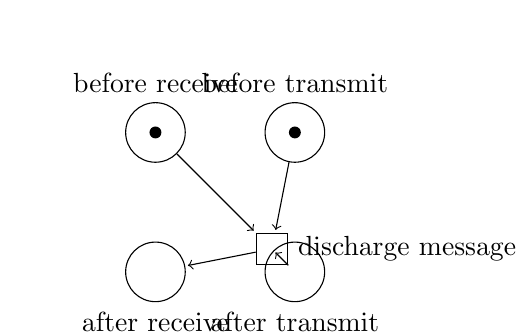
\begin{tikzpicture}
  \node[place,tokens=1,label=above:{before receive}] (beforeRx) {};
  \node[place,tokens=1,right = of beforeRx, label=above:{before transmit}] (beforeTx) {};
  \node[place,tokens=0,below=of beforeRx, label=below:{after receive}] (afterRx) {};
  \node[place,tokens=0,below=of beforeTx, label=below:{after transmit}] (afterTx) {};
  \node[transition,below right=of beforeRx, label=right:{discharge message}] (trans) {}
  edge [pre] (beforeRx)
  edge [pre] (beforeTx)
  edge [post] (afterRx)
  edge [post] (afterTx);
\end{tikzpicture}

Discharging a message here means copying the relevant bits of state from the transmitting thread's local state into the receiving thread's local state.
A message can be discharged if there is one thread willing to send it and one thread willing to receive it.
While the message is being discharged the two threads are effectively merged, with only one thread actually executing the message side effects.
Once the message is finished the two threads separate again and continue to execute independently.

A thread is only willing to receive a message if the message would pass the thread's message filter.
This has two parts:

\begin{itemize}
\item
  The message must have the correct message ID.
  This simply means that the send and receive parts of the message operation must be trying to enforce the same happens-before edge.
\item
  The message must pass the receiving thread's message receive filter.
  This filter consists of all of the side-conditions present in the crash enforcement plan which will become evaluatable once the message has been received.
\end{itemize}

However, in a real implementation, the threads are not pre-specified, and most of the complexity of the message algorithm lies in determining them.
When the plan demands that a message be sent or received, one side can be determined trivially, but the other must be discovered.
For a receive operation, the algorithm to do so in the abstract semantics looks like so:

\begin{algorithmic}[1]
  \IF {$l$ has a bound thread}
    \IF {The bound thread does not have an outgoing message}
      \STATE {Wait for it to send one}
    \ENDIF
    \IF {The bound thread has an outgoing message and it passes the message filter}
      \STATE {Discharge the message}
    \ELSE
      \STATE {$l$ has failed; remove it from the active set}
    \ENDIF
  \ELSE
    \STATE {Examine the set of outstanding unbound message sends and collect all of the ones which pass the message filter into $s$}
    \STATE {Extend $s$ with $\bot$}
    \STATE {Choose $s'$ non-deterministically from $s$}
    \IF {$s\prime = \bot$}
      \STATE {Register $l$ as a receiver of unbound messages}
      \STATE {Wait for the delay specified in this receive operation}
      \STATE {Unregister $l$ as a receiver of unbound messages}
      \STATE {Collect all of the unbound sends which pass the filter which started while we were waiting into $s$}
      \STATE {Select $s'$ non-deterministically from $s$}
    \ENDIF
    \STATE {Discharge $s'$}
  \ENDIF
\end{algorithmic}

The send operation is symmetric:

\begin{algorithmic}[1]
  \IF {$l$ has a bound thread}
    \IF {The bound thread is attempting to receive a message}
      \STATE {Wait for it to start receiving}
    \ENDIF
    \IF {The bound thread is receiving a message and this message would pass its filter}
      \STATE {Discharge the message}
    \ELSE
      \STATE {$l$ has failed; remove it from the active set}
    \ENDIF
  \ELSE
    \STATE {Examine the set of outstanding unbound message receives and collect all of the ones whose filters this message would pass into $s$}
    \STATE {Extend $s$ with $\bot$}
    \STATE {Choose $s'$ non-deterministically from $s$}
    \IF {$s' = \bot$}
      \STATE {Register $l$ as a sender of unbound messages}
      \STATE {Wait for the delay specified in this receive operation}
      \STATE {Unregister $l$ as a sender of unbound messages}
      \STATE {Collect all of the unbound receives whose filters this message would pass which started while we were waiting into $s$}
      \STATE {Select $s'$ non-deterministically from $s$}
    \ENDIF
    \STATE {Discharge $s'$}
  \ENDIF
\end{algorithmic}

As shown in figure ..., each message operation effectively defines an interval in time, and a send and receive match up if these windows overlap.
The behaviour when $s' = \bot$ is perhaps somewhat surprising: the thread waits a little while and then selects a peer thread to discharge the message with non-deterministically.
Meanwhile, all of the other threads are simultaneously performing similar non-deterministic choices.
The use of look-ahead nondeterminism means that all of the threads will make these selections in a mutually compatible way, so that there is no danger of A attempting to discharge its message with B while B discharges with C.
The actual implementation must resolve these constraints much more carefully, and is discussed in detail later.

Note that the message receive filter is evaluated as the message is being discharged, while the two threads are merged.
It is possible to imagine an alternative implementation in which the filter is instead evaluated locally in the receiver after the discharge operation is complete.
This would reduce the size of the synchronised section and so would appear, on the face of it, to offer greater parallelism, and hence potentially better performance.
Unfortunately, it does not work.
To illustrate the problem, consider again the example shown in figure \todo{...}.
One thread modifies a shared structure while another thread reads it, and the program will crash if the two threads happen to be operating on the same structure at the same time.
Suppose that the read thread runs far more often than the write one and that there are many instances of the structure.
The timeout balancing logic will quickly reduce the delay on the read side's first message send to zero and increase the delay on the write side's first message receive to compensate.
Now, when the write thread does run, it will stop just before \verb|l9| waiting for a matching read thread to arrive.
By hypothesis, many such threads will arrive, as the read thread runs more often than the write one.
In the alternative design, the read thread cannot evaluate the write thread's receive filter, and so every read thread will attempt to bind to the write thread, forcing the write thread to be duplicated many times.
Because of timeout rebalancing, the read thread will proceed from \verb|l2| immediately and quickly reach \verb|l5|, where it has to receive a message from \verb|l9|.
At this point, there are two possible outcomes:

\begin{itemize}
\item
  The thread is delayed at \verb|l5| waiting for the message from \verb|l9|.
  The write thread is still waiting in case any other threads reach \verb|l2| and attempt to synchronise with it, and so this might potentially be a rather long delay.
  Since the read thread runs far more often than the write thread, this will have a very large performance impact.
  Worse, it will probably be pointless: there, by hypothesis, a large number of instances of the structure which is being examined, and so, with high probability, the write thread will be modifying a different one.
  When the write thread does finally escape from its receive delay and evaluate its receive filter it will discover that the filter fails, and so the write thread will exit.
  The read thread will then discover that its bound thread has exited and be forced to exit as well.
  The crash enforcement plan will therefore not complete and the bug is highly unlikely to reproduce.
  
  Even worse, the performance hit might mean that the read thread will run far less frequently, further reducing the likelihood of the bug reproducing.
  In extreme cases, the attempt at enforcing a crash might actually make the bug less likely to reproduce in unit time.
\item
  The thread is not delayed at \verb|l5|.
  It never receives the message from \verb|l9| and must therefore exit without completing the plan, so is unlikely to reproduce the bug.
  The write thread's high-level interpreter will then accumulate a collection of low-level threads which have bound to exited read threads and which will themselves immediately exit.
\end{itemize}

Neither outcome helps to reproduce the target bug.

By contrast, in the scheme used by SLI, the read thread is able to evaluate the write thread's message receive filter at \verb|l2|.
It will therefore only bind to write threads which modify the structure which it is reading.
That means that the thread can be delayed a relatively long time at \verb|l5| without fear of apocalyptic performance damage, and so the bug will reproduce relatively easily.

\subsubsection{Discuss the timeout balancing bit}

\subsubsection{Implementing non-deterministic choice in the Succ phase}

It might be that an instruction has several possible successors in the control flow graph in the crash execution plan, and in that case the interpreter must choose one of these successors using look-ahead non-determinism.
This cannot be implemented in any physically-realisable system, as it is non-causal, and so SLI must emulate it.
SLI uses a power-set construction to do so.
Rather than operating a single interpreter context, the actual implementation maintains a set of low-level interpreter contexts, which roughly follow the abstract semantics given above, and interprets them all in lock-step parallelism.
When one of these low-level interpreters needs to perform a non-deterministic choice between $n$ possible values, the high-level interpreter creates $n$ successor low-level interpreter states, one corresponding to each possible outcome of the choice, and inserts all of them into its current-state set.
They are then interpreted in parallel until enough information is available to resolve the earlier choice, at which point all but one of the threads will exit and the interpreter can revert to single-threaded execution.
If a thread is bound when it performs a non-deterministic choice then its bound thread must also be duplicated, to ensure that the new thread has something to bind to.

One subtlety here is that the original program's underlying instruction can only be retired once, and so the high-level interpreter must ensure that all low-level interpreters arrive at that point in the execution cycle at the same time.
SLI actually enforces a slightly stronger constraint, which is that every low-level interpreter in a given high-level interpreter must be at the same phase in the instruction execution cycle.
The only phases for which this is difficult are the message send and receive phases, which are discussed in more detail in the next section.

\subsubsection{Concrete implementations of message send and receive}

The message receive operation looks like this:

\begin{algorithmic}[1]
  \STATE {$lls \gets $ the set of currently-active low-level interpreter states}
  \STATE {$newLls \gets $ an empty set of low-level interpreter states}
  \FORALL {$l$ in currently-active low-level interpreter states}
    \IF {$l$ does not receive any messages}
      \STATE {Move $l$ from $lls$ to $newLls$ without changing it}
    \ELSIF {$l$ has a bound thread}
      \IF {$l$'s bound thread has exited}
        \STATE {$l$ exits as well; remove it from $lls$ without adding it to $newLls$}
      \ELSIF {$l$'s bound thread has an outgoing message}
        \IF {The bound thread's outgoing message passes the message filter}
          \STATE {Copy stashed values from the sending low-level interpreter's state to the receiving one}
          \STATE {Move $l$ from $lls$ to $newLls$}
        \ELSE
          \STATE {$l$ exits; remove it from $lls$}
        \ENDIF
      \ELSE
        \STATE {} \COMMENT {Wait for a the bound thread to send a message}
      \ENDIF
    \ELSE
      \STATE {} \COMMENT{Unbound receive}
      \FORALL {$s$ registered unbound senders}
        \IF {$s$'s outgoing message passes the message filter}
          \STATE {$l' \gets $ duplicate $l$}
          \STATE {$s' \gets $ duplicate $s$}
          \STATE {Copy stashed values from $s'$'s state to $l'$'s}
          \STATE {Bind $l'$ and $s'$ together}
          \STATE {Insert $l'$ into $newLls$}
          \STATE {Insert $s'$ into $s$'s high-level interpreter's active low-level interpreter list}
        \ENDIF
      \ENDFOR
      \STATE {Register $l$ as an unbound receiver}
    \ENDIF
  \ENDFOR

  \IF {$lls$ is empty}
    \RETURN
  \ENDIF

  \STATE {$end \gets now() + bound\_delay$}
  \IF {There is a minimum delay}
    \STATE {Release lock}
    \STATE {Sleep for the minimum delay}
    \STATE {Acquire lock}
  \ENDIF

  \WHILE {There are bound receives in $lls$ and $now() < end$}
    \STATE {Release lock}
    \STATE {Wait for some bound receive to complete, or for the current time to pass $end$}
    \STATE {Acquire lock}
    \FORALL {$l$ performing bound receives in $lls$}
      \IF {$l$'s bound thread has exited}
        \STATE {Remove $l$ from $lls$}
        \STATE {$l$ exits}
      \ELSIF {$l$'s receiving-bound-message flag is clear}
        \STATE {Remove $l$ from $lls$}
        \STATE {Add $l$ to $newLls$}
      \ELSE
        \STATE Continue waiting
      \ENDIF
    \ENDFOR
  \ENDWHILE

  \FORALL {$l$ in $lls$}
    \IF {$l$ is registered as an unbound receiver}
      \STATE {Unregister $l$ as an unbound receiver}
    \ENDIF
    \IF {$l$ was attempting a bound receive and the bound thread hasn't sent any messages}
      \STATE {Exit $l$}
    \ELSIF {$l$ is unbound}
      \STATE {The thread must have been attempting an unbound receive which failed, so exit $l$}
    \ELSE
      \STATE {} \COMMENT {Receive succeeded}
      \STATE {Add $l$ to $newLls$}
    \ENDIF
  \ENDFOR

  \STATE {Set high-level interpreters set of currently-active low-level interpreters to $newLls$}
\end{algorithmic}

The send algorithm is very similar:

\begin{algorithmic}[1]
  \STATE {$lls \gets $ the set of currently-active low-level interpreter states}
  \STATE {$newLls \gets $ an empty set of low-level interpreter states}
  \FORALL {$s$ in currently-active low-level interpreter states}
    \IF {$s$ does not send a message}
      \STATE {Move $l$ from $lls$ to $newLls$ without changing it}
    \ELSIF {$s$ has a bound thread}
      \IF {$s$'s bound thread has exited}
        \STATE {$s$ exits as well; remove it from $lls$ without adding it to $newLls$}
      \ELSIF {$s$'s bound thread is waiting to receive a message}
        \IF {$s$'s outgoing message passes the message filter}
          \STATE {Copy stashed values from the sending low-level interpreter's state to the receiving one}
          \STATE {Move $s$ from $lls$ to $newLls$}
          \STATE {Clear the bound thread's receiving-bound-message flag}
        \ELSE
          \STATE {$s$ exits; remove it from $lls$}
        \ENDIF
      \ELSE
        \STATE {} \COMMENT {Wait for a the bound thread to be ready to receive a message}
      \ENDIF
    \ELSE
      \STATE {} \COMMENT{Unbound send}
      \FORALL {$l$ registered unbound receivers}
        \IF {The outgoing message passes $l$'s message filter}
          \STATE {$l' \gets $ duplicate $l$}
          \STATE {$s' \gets $ duplicate $s$}
          \STATE {Copy stashed values from $s'$'s state to $l'$'s}
          \STATE {Bind $l'$ and $s'$ together}
          \STATE {Insert $s'$ into $newLls$}
          \STATE {Insert $l'$ into $l$'s high-level interpreter's active low-level interpreter list}
        \ENDIF
      \ENDFOR
      \STATE {Register $s$ as an unbound sender}
    \ENDIF
  \ENDFOR

  \IF {$lls$ is empty}
    \RETURN
  \ENDIF

  \STATE {$end \gets now() + bound\_delay$}
  \IF {There is a minimum delay}
    \STATE {Release lock}
    \STATE {Sleep for the minimum delay}
    \STATE {Acquire lock}
  \ENDIF

  \WHILE {There are bound sends in $lls$ and $now() < end$}
    \STATE {Release lock}
    \STATE {Wait for some bound send to complete, or for the current time to pass $end$}
    \STATE {Acquire lock}
    \FORALL {$s$ performing bound sends in $lls$}
      \IF {$s$'s bound thread has exited}
        \STATE {Remove $s$ from $lls$}
        \STATE {$s$ exits}
      \ELSIF {$s$'s sending-bound-message flag is clear}
        \STATE {Remove $s$ from $lls$}
        \STATE {Add $s$ to $newLls$}
      \ELSE
        \STATE Continue waiting
      \ENDIF
    \ENDFOR
  \ENDWHILE

  \FORALL {$s$ in $lls$}
    \IF {$s$ is registered as an unbound sender}
      \STATE {Unregister $s$ as an unbound sender}
    \ENDIF
    \IF {$s$ was attempting a bound send and the bound thread hasn't tried to receive any messages}
      \STATE {Exit $s$}
    \ELSIF {$s$ is unbound}
      \STATE {The thread must have been attempting an unbound send which failed, so exit $s$}
    \ELSE
      \STATE {} \COMMENT {Send succeeded}
      \STATE {Add $s$ to $newLls$}
    \ENDIF
  \ENDFOR

  \STATE {Set high-level interpreters set of currently-active low-level interpreters to $newLls$}
\end{algorithmic}

One further optimisation, not shown here, avoids redundantly duplicating low-level interpreter contexts in the common case that a message operation is discharged precisely once.

\todo{Discuss setting minimum delays here}

\subsubsection{The await-bound-thread-exit state}

When a thread completes its plan, it is sometimes useful for it to wait for its bound thread to exit before proceeding.
This is because the crash summary from which the plan is generated does not have complete information on the structure of the program.
If the last edge in a happens-before graph is from memory access A to memory access B, that generally means that A is a store and B is a load and B must load the value stored by A.
That means that, not only must B happen after A, but B must happen before any other writes to the memory location modified by A.
If there were other stores to that location in the crash summary then the happens-before graph would include additional edges to ensure that that happens, but if there are stores outside of the summary then it will not.
For instance, suppose that the write thread looks like this:

\begin{verbatim}
while (1) {
l1:  *x = 5;
l2:  *x = 7;
     <something_complicated>
}
\end{verbatim}

And the read thread looks like this:

\begin{verbatim}
l3: a = *x;
l4: b = *x;
    crash if a != b;
\end{verbatim}

This program is clearly buggy.
One way of reproducing this bug would be to interleave instructions as \verb|l1|, \verb|l3|, \verb|l2|, \verb|l4|.
SLI will discover this interleaving as the happens-before graph show in figure \todo{...}.
The algorithm described so far will be sufficient to enforce this graph (assuming that the two fragments of code shown can actually execute in parallel).
This is not, however, sufficient to cause the program to crash, because the generated happens-before graph is incomplete: it misses the edge from \verb|l4| to \verb|l1| in the next iteration of the loop.
If the loop completes and reaches the store at \verb|l1| before the load \verb|l4| completes then the bug will not reproduce even though the happens-before graph was successfully enforced.
Any scheme with an analysis horizon based on a simple instruction count will suffer from a similar problem, but this is particularly serious for SLI, because the delays inserted are in almost precisely the right place to maximise the chance of this kind of bug-hiding race.
Returning to the example, SLI's crash enforcement plan will include a delay after \verb|l1| (to implement the \verb|l1| to \verb|l3| happens-before edge), and this delay will be large relative to a short sequence of normal instructions, and so the bug will be hidden completely provided that the delay to wake up the read thread after the final edge is greater than the time taken to execute \verb|<something_complicated>|.
This is perfectly plausible, given that \verb|<something_complicated>| only needs to be a few dozen instructions to exceed SLI's analysis window.
This bug will therefore never reproduce under SLI's crash enforcer, even when the happens-before graph is enforced perfectly.
The fix is simple: have the store thread delay slightly after completing its final message send operation, until the read thread also completes its crash enforcement plan.
This ensures that activity beyond the analysis horizon cannot prevent bug reproduction, and, because it only happens when the plan is mostly complete, and hence happens very rarely, it has very low performance overhead.

\begin{tikzpicture}
\node[CfgInstr] (l1) {l1};
\node[CfgInstr, below = of l1] (l2) {l2};
\node[CfgInstr, right = of l1] (l3) {l3};
\node[CfgInstr, below = of l3] (l4) {l4};
\draw[->] (l1) -- (l2);
\draw[->] (l3) -- (l4);
\draw[->,happensBeforeEdge] (l1) -- (l3);
\draw[->,happensBeforeEdge] (l3) -- (l2);
\draw[->,happensBeforeEdge] (l2) -- (l4);
\end{tikzpicture}


\subsubsection{Compiling the plan}

In addition to a plan interpreter, SLI also includes a plan compiler, which combines the plan with the program's original machine code to produce a modified version of the program which performs the necessary enforcement actions without needing an interpreter.
The intent here is to reduce the overhead of the interpreter in the case where SLI is investigating many bugs most of which do not exist.
Making this practical requires several simplifications to the semantics:

\begin{itemize}
\item
  The number of physical program threads operating in the plan is limited.
  In particular, it is assumed that only one program thread will be executing the read side of the plan at any time, and likewise only one thread will be executing the write side.
\item
  The message semantics are simplified: messages are sent asynchronously, with a delay only on the read side, and must be ``cancelled'' when the relevant thread exits.
  This has two important implications: first, that a message send can never fail and, second, the something must keep track of what messages a given thread currently has outstanding.
  Combined with the first simplification, it also means that at most one instance of any given message can be outstanding at any one time, and so it is easy to place the relevant information in a global structure without needing any dynamic memory allocation.
\item
  High-level interpreter contexts only ever access the state of their own low-level interpreters.
  This has two important implications:

  \begin{itemize}
  \item
    Remote low-level interpreters are never duplicated during message operations.
    If the normal semantics would require an interpreter to be duplicated then the local message operation fails.
  \item
    The receive message filter can only be executed by the receiving thread after receiving a message.
  \end{itemize}
\item
  When a low-level interpreter is duplicated due to a non-deterministic choice in the Succ phase the low-level state's stash table is not duplicated.
  Instead, all low-level interpreters in a given high-level interpreter share a single stash table.
\end{itemize}

The result is a system with lower run-time overheads, but also a lower probability of reproducing interesting bugs.
It has a much larger I-cache footprint but a smaller D-cache one\editorial{Not sure where I'm going with that, although it is true and kind of interesting}.

I now briefly outline the implementation of this compiler.
The core idea is to compile the CFG in the enforcement plan into a state machine.
This state machine consists of a large number of smaller intra-instruction state machines, as illustrated in figure~\todo{...}, each of which models a single instruction in the original program.
The label on each state is itself a set of low-level labels which consist of a four-tuple of the plan thread which is executing, a reference to the plan CFG node, a set of messages which have been sent by the thread, and the phase of the intra-instruction state machine.
Each state is compiled to a small fragment of machine code (which might be empty, if this instruction does not have an relevant annotation in the plan) plus a set of relocations specifying the fragment's relationships to the other states.
Once every state has been compiled these relocations can be discharged and the fragments concatenated together to form the final patch.

I now discuss the details of each phase of the intra-instruction machine:

\begin{itemize}
\item[RecvMsg]
  Examine the set of CFG nodes which are active in the current state and determine whether the plan requires any of them to receive messages.
  If so, emit code to examine the global outstanding-message structures to see whether of the desired messages are currently outstanding.
  If there are, receive precisely that message.
  Any other message receive operations are considered to have failed and the relevant CFG nodes removed from the current state label.
  If no message sends are currently outstanding then the physical thread is delayed until either one is available or some timeout is reached.
  If a message becomes available then it is received, and otherwise all receives fail and all receiving CFG nodes are removed from the label.
  Note that this does not necessarily mean that the state label will become empty\footnote{Although that is the common case.} as there may be some CFG nodes which do not need to receive messages.

  Once a message is received its content is simply copied from the global message area into the local thread's stash area.
\item[OrigInstr]
  Store any generated values into simulation slots and issue the original instruction.
  There are three main cases to consider here:

  \begin{itemize}
  \item
    Simple memory loads.
    If the instruction is of the form \verb|LOAD *location -> register|, and the value loaded is to be saved, then it is sufficient to just copy \verb|register| into the simulation slot after the original instruction has completed.
  \item
    Compound memory loads.
    Instructions which load from memory but are not themselves simple loads are more difficult to handle.
    For concreteness, suppose that the instruction is \verb|CMP 76,*loc1|, and the annotation requires us to save the value loaded.
    The instruction loads from \verb|*loc1| but does not leave the result in any locations which we can easily access.
    It would be possible to solve this problem by adding another load of \verb|*loc1|, but that would run the risk of a store in a remote thread modifying \verb|*loc1| between the two loads, leading to very confusing results.
    SLI instead solves this problem by rewriting the instruction to this:

\begin{verbatim}
LOAD *loc1 -> reg1
STORE reg1 -> simslot
CMP 76, reg1
\end{verbatim}

    This exposes the loaded value to the instrumentation framework, allowing it to be stored to the simulation slot as desired.

    Instructions which modify memory in-place, such as \verb|ADD 1 + *loc1 -> *loc1|, pose a similar problem and can be solved in the same way, provided that they do not have a \verb|LOCK| prefix.
    \verb|LOCK|ed instructions are more complex, as separating the load and store phases into separate instructions would violate the semantics of the program and might introduce new bugs.
    SLI solves this problem using a \verb|CMPXCHG| loop.
    For instance, the instruction \verb|LOCK ADD 1 + *loc1 -> *loc1| would be converted to this machine code fragment:

\begin{verbatim}
1: LOAD *loc1 -> reg1
ADD 1 + reg1 -> reg2
LOCK CMPXCHG *loc1, reg1 -> reg2
if_cmpxchg_failed goto l1
STORE reg1 -> simslot
\end{verbatim}

    The \verb|CMPXCHG| instruction here is supposed to be an invented syntax for the x86 machine code instruction which atomically compares \verb|*loc1| to \verb|reg1| and, if they are equal, sets \verb|*loc1| to \verb|reg2|.
    This allows SLI to expose the value of the implicit load while preserving the \verb|LOCK| semantics of the original instruction.
  \item
    Branch instructions are deferred to the FindSucc state.
  \end{itemize}
  
\item[SendMsg]
  Send any outgoing messages.
  This amounts to simply copying the message payload into the global message area, setting a global flag to indicate that the message is currently outstanding, and adding the message ID to the state label's set of sent messages.
  This always succeeds and advances to the FindSucc state.

\item[ExitThread]
  When a low-level thread exits it is necessary to cancel any messages which it has sent.
  The compiler takes the union of all of the sent-messages sets in its low-level, removes the thread which is to exit, and then takes the union again.
  Any messages present in the first set but not the second need to be cancelled by setting the relevant global message-outstanding flag to zero.
  The compiler will then either exit the patch, if the last low-level thread has exited, or resume the intra-instruction state machine at an appropriate place.
\end{itemize}


\begin{tikzpicture}
\node[flowChartState] (RecvMsg) {RecvMsg};
\node[flowChartState,above left = of RecvMsg] (StartThread) {StartThread};
\node[flowChartState,above right = of RecvMsg] (CheckForThreadStart) {CheckForThreadStart};
\node[flowChartState, below = of RecvMsg] (OrigInstr) {OrigInstr};
\node[flowChartState, below = of OrigInstr] (VerfCond) {VerfCond};
\node[flowChartState, below = of VerfCond] (SendMsg) {SendMsg};
\node[flowChartState, below = of SendMsg] (FindSucc) {FindSucc};
\node[flowChartState, right = of VerfCond] (CondFail) {CondFail};
\node[flowChartState, right = of CondFail] (Exit) {Exit};
\node[flowChartState, left = of RecvMsg] (RecvdMsg) {RecvdMsg};
\draw[->] (CheckForThreadStart) -- (RecvMsg) -- (OrigInstr) -- (VerfCond) -- (SendMsg) -- (FindSucc);
\draw[->] (StartThread) to [bend right=10] (CheckForThreadStart);
\draw[->] (CheckForThreadStart) to [bend right=10] (StartThread);
\draw[->,dashed] (FindSucc.east) to [bend right=75] (CheckForThreadStart.east);
\draw[->] (RecvMsg) -- (RecvdMsg) -- (OrigInstr);
\draw[->] (RecvMsg) -- (Exit);
\draw[->] (VerfCond) -- (CondFail) -- (Exit);
\draw[->] (FindSucc) -- (Exit);
\end{tikzpicture}

  

\subsubsection{Compiling entry point stubs}


\subsubsection{Run-time considerations}

Recovery from spurious segfaults in the patch due to e.g. LD operations.

\subsection{Comparison to schedule memoisation}
\subsection{Comparison to STM block inference stuff}

\section{Fixing bugs}

\subsection{Using global locks}
\subsection{Using message passing}

\chapter{Other modes of operation}
\section{Building \StateMachines from DRS logs}
The simplest way to fix a bug is to start from a DRS log.
Given a log, identifying the thread and which is most responsible for a crash is generally straightforward.
If the crash is caused by dereferencing a bad pointer then the responsible thread is the one which dereferenced the pointer; if the crash is an assertion failure then the responsible thread is the one which called \verb|abort()| (or equivalent).
The log then makes it trivial to determine what instructions the responsible thread executed before it crashed, and a suffix of these can be compiled into a \StateMachine capturing the most relevant parts of the responsible thread's behaviour.


\subsection{Requirements on the DRS}
\section{Building \StateMachines from crash dumps}
\section{Turning a collection of \StateMachines into a fix}

\chapter{Analysis on \StateMachines}
\section{Alias analysis}
\subsection{Alias analysis and identification of thread-local accesses}
There are two major complications to optimising memory accesses:

\begin{itemize}
\item
  Alias analysis.
  Most memory-related optimisations rely on being able to tell whether two pointers alias with each other.
  This is impossible in the general case, but it is possible to develop some useful (sound and unsound) approximations.
  This is very similar to the problem of the same name faced by optimising compilers, except that optimising compilers generally have more information (e.g. type information).
\item
  Checking whether an access is thread-local.
  Most races are mediated through memory, and all of the races targeted by SLI will involve some memory-accessing component.
  Correctly handling races restricts the available space of optimisations, often substantially.
  For instance, if a machine stores to a location and then immediately loads from it again then it might be tempting to forward the stored expression to the load, but this is invalid if another thread might store to the same location in between the two accesses.
  This is a common cause of races, and one which can be easily handled by SLI-like techniques, and so it is important not to eliminate it at the machine simplification stage.
\end{itemize}

If a DRS log is available then this is generally trivial, as all of the necessary information will be present in the log\editorial{should really have a ref to the DRS section, which'll have more details.}.
Otherwise, SLI uses a combination of static and dynamic analyses to solve these problems.

\subsubsection{Dynamic analysis}

The most important technique used by SLI is a dynamic analysis which is used before starting static analysis to build a model of how the program behaves.
This attempts to classify the memory-accessing instructions in the program according to which other memory accesses they might alias with and whether the memory accesses appears to be private to that thread.
The result is an aliasing database which consists of a set of aliasing entries.
Each aliasing entry consists of a pair of sets of instructions, with one set containing loads and the other stores, with each instruction tagged with a bit saying whether the accessed memory was thread-local or possibly-shared.
The database is generated using a dynamic analysis implemented as a Valgrind skin.

\todo{Should really describe how the skin works.  Mostly just an engineering detail, though.}

\todo{The bit where we figure out whether a dynamic pointer is thread-private is kind of interesting, though.}

Given this database, it is generally possible to eliminate the vast majority of possibly-aliasing pairs quickly, which means that the aliasing problem becomes much simpler.
Of course, it is only correct if the dynamic execution completely captures every possible behaviour of the program.
This is a particular concern if the program is misbehaving, as such misbehaviour might lead to wild pointer-type bugs, or uses after free, or a number of other bugs, which would mean that the afflicted instructions could potentially alias with almost any other memory-accessing instruction in the program, and this would not be accurately reflected in the aliasing database.

\todo{Should really say something more about that}

This database does not include accesses to the local stack, in order to keep its size down to something reasonable.

\subsubsection{Accesses to the current stack frame}

The dynamic aliasing database does not include any information on accesses to the current thread's stack, and so SLI needs to employ a different mechanism to determine aliasing relations for those accesses.
Most such accesses take the form of constant offsets from \verb|RSP| (or \verb|RBP|, which is converted to a \verb|RSP| offset as discussed in \S\ref{sect:rbp_canonicalisation}), and these can be handled trivially.
More interesting are cases where pointers to stack-allocated objects are stored into other registers.
These are moderately rare\editorial{Numbers?}, but, when they do occur, tend to cause significant complications for the other analysis passes, as stores to those objects cannot be easily shown to be independent of independent accesses.
For instance, suppose that SLI had derived a machine fragment like so:

\begin{verbatim}
STORE t1 -> RSP + 8 @ A
STORE t2 -> RBX     @ B
LOAD  t3 <- RSP + 8 @ C
\end{verbatim}

and that \verb|RBX| in this cases points at the local stack.
Neither the dynamic aliasing database nor simple peephole alias checking will be able to show that \verb|A| and \verb|B| do not alias, and so it will not be possible to forward the store at \verb|A| to the load at \verb|C|.
In larger examples this can cause significant problems.

Most such non-\verb|RSP| stack pointers point outside of the current stack frame (usually because the calling function has allocated a local variable and then passed in a pointer to it), as the compiler will generally emit \verb|RSP|- or \verb|RBP|-relative accesses for most local variables.
SLI therefore uses a static points-to analysis to classify registers according to where they point:

\begin{itemize}
\item
  The current function's stack frame.
\item
  Outside the current function's stack frame.
  This could be a calling function's frame, the heap, statically allocated data, or somewhere else entirely.
\item
  Nowhere at all.
  The register is not a valid pointer.
  Strictly speaking, this could be treated as a pointer outside of the current frame, but splitting the state out like this does not complicate the analysis and can provide marginally better results in some corner cases.
\end{itemize}

Each combination of register and static instruction is assigned some subset of those classifications representing the possible dynamic values of the register.
Static instructions are also assigned a flag indicating whether any pointers to the current stack frame have escaped i.e. been stored to memory outside of the stack frame.
If the stack has not escaped then loads can be assumed to return something which does not point to the current frame; otherwise, any loaded pointer might be a stack pointer.
\editorial{Could do better than this with a more complete analysis, but I really don't care all that much.}

The static analysis is, at its core, an iteration to a fixed point applied independently to each function.
In the initial state, the entrypoint instruction of the function is assigned a configuration in which \verb|RSP| is definitely a pointer to the current frame and every other register is either not a pointer or a pointer outside of the current frame.
Other instructions start with a bottom configuration: no registers are assigned any classification, and the stack pointer is considered not to have escaped.

\todo{The update step is pretty damn obvious, but I should probably describe it explicitly for completeness.}

\todo{Once the iteration has converged, any un-visited instructions have their bottom configuration replaced by a top configuration, in which any aliasing relationships are possible.  Not entirely convinced that's a good idea; I suspect it's just going to hide bugs.}

As usual, called functions are assumed to be pure, in the sense that they compute some function of their arguments and return it in a well-known register, with no other side-effects.
The return register is considered to possibly contain a stack pointer if any of the arguments to the function possibly contain a stack pointer.
If the call has multiple possible targets then each is considered in turn, and the result is the join of all of the results of the individual callable functions.
\todo{Explain how I determine the possible targets.}
\todo{Explain how I determine what arguments a function has.}
\todo{This is unsound only because of the way we handle escaped stack pointers.  Doing it properly would be trivial, but would make the analysis less effective.  Should collect numbers on how bad it would be.}

The underlying assumption here is essentially that the program to be analysed follows a broadly normal calling convention where local variables cannot be accessed until the relevant function is invoked, and must not be accessed after the function returns.
There is also an assumption that the analysis can correctly determine the entry points of functions, and that every instruction is part of precisely one function\editorial{Really need to explain how we define functions in the presence of tail calls.}.
That ensures that, at the start of a function, no pointers to function-local variables can exist anywhere in the program's address space or register state, except for the stack pointer itself.
Assuming that that assumption is correct, this analysis is sound, except for the handling of called functions.

The result of this analysis is a map which classifies every combination of static instruction and register name according to what type of memory (current stack frame, other memory, or invalid memory) it points to.
This allows the alias analysis to rapidly eliminate the vast majority of aliasing checks comparing accesses to local variables to accesses to other types of memory, which is a significant win\editorial{blah}.

\subsubsection{Fallback resolution}
When neither the dynamic nor local-frame static analyses can answer an aliasing question, SLI attempts to resolve it using a peephole resolver.
To check whether \verb|A| and \verb|B| might possibly refer to the same memory location, SLI generates the expression \verb|A == B| and then passes it to the expression simplifier (see \S\ref{sect:peephole_simplification_expressions}).
If the result is the constant \verb|1| then \verb|A| and \verb|B| definitely alias; if it is the constant \verb|0| then they definitely don't; and otherwise they might alias and might not.
In the last case alias analysis, finally, fails.
Depending on the intended use of the alias result, SLI will then either choose a safe default or use a case split to consider both possibilities.

\section{Static analysis-based simplifications}
\section{Discussion of the SSA form used}
Because it's very subtly different from the form most commonly used in optimising compilers.
Also worth talking about the use of SDA form here as well.

\section{Other simplifications}
\subsection{Dead register elimination}
\todo{I suspect I'm being a bit condescending describing this at all, much less giving it this many words.}

SLI is generally only interested in a small part of the program's behaviour.
This means that many of the values computed by the program will be completely irrelevant and can be safely eliminated.
Dead register elimination is one of the simplest ways of doing so.
In this pass, SLI examines the generated machine to discover temporary variables whose values are never used, and then eliminates them completely.
It is analogous to the dead code elimination pass of an optimising compiler.

As an example, suppose that the original program looked like this:

\begin{verbatim}
*ptr = global_variable1->field1->field2 + global_variable2;
\end{verbatim}

This might generate machine code like this:

\begin{verbatim}
A:  load ptr -> rsi
B:  load global_variable1 -> rax
C:  load (rax + offsetof(field1)) -> rax
D:  load (rax + offsetof(field2)) -> rax
E:  load global_variable2 -> rdx
F:  add rdx + rax -> rax
G:  load rax -> (rsi)
\end{verbatim}

and SLI is attempting to investigate a possible crash caused by \verb|rsi| being a bad pointer at \verb|G|.
The first approximation machine generated might be (after conversion to SSA):

\begin{verbatim}
@A:
l1: LOAD ptr -> rsi:0
    LOAD global_variable1 -> rax:0
    LOAD (rax:0 + offsetof(field1)) -> rax:1
    LOAD (rax:1 + offsetof(field2)) -> rax:2
    LOAD global_variable2 -> rdx:0
    COPY rax:3 <- rax:2 + rdx:0
    l2
l2: if (BadPtr(rsi))
    then l3
    else l4
l3: <crash>
l4: <survive>
\end{verbatim}

Most of the loads can have no possible effect on the outcome of the machine, as the value loaded can never reach the condition of the \verb|l2| state\footnote{Assuming that they do not themselves dereference bad memory, of course.  However, if they do, the crash of interest will not occur, and so that case can be at some level ignored.}.
In that sense, they are dead, and should be removed.

The algorithm used for doing so has two parts.
In the first, the machine is examined to determine where each variable is live using a straightforward Tarski-style fixed-point iteration.
In the second, any definitions of variables which are never used are eliminated.

The Tarski iteration works by building up a mapping from machine states to sets of variables which are valid at the start of that state.
In the initial state, anything referenced by the free variables table is considered to be valid everywhere (see~\ref{sect:freevars}), and anything else is considered to be dead everywhere.
The update rule proceeds by propagating liveness information backwards through machine edges until it reaches the start of the edge, marking variables live when they are used and dead when they are assigned to.
Meets in the state graph are handled by taking the union of the liveness information at the starts of all of the successor edges.
This process iterates until it converges.
At that point, the analysis has a mapping from locations in the state machine to the set registers which are live at those locations, and given that it is trivial to determine which side effects are dead and to eliminate them.

This optimisation has a pleasant cascading property: when a side-effect is eliminated, it will no longer keep its inputs live, which can cause them to become dead.
That often causes further side effects to become dead, and so allow more of the machine to be eliminated.
This allows this very simple optimisation to sometimes eliminate\editorial{si} large amounts of the machine.

\subsection{Register copy propagation}
\todo{I'm basically restating how Cifuentes' register copy propagation algorithm works here, which might be a bit of a waste of time.  Expand on it later on, though, so having the details here helps a bit.}

Compiling a high-level language into machine code requires complex expressions to be broken down into a series of smaller operations.
SLI then examines the resulting sequence of small operations, and this tends to lead to approximation machines with a large number of intermediate temporary values each of which stores the result of a very simple calculation.
Later analysis phases are generally more straightforward if these simple expressions are re-combined into one larger one.
For instance, a C program like this:

\begin{verbatim}
x = (y * 32 + z / 8) % (y + 2);
\end{verbatim}

might compile into machine code\footnote{This is intended to be a representation of x86 machine code.  It is somewhat more explicit than the usual Intel or AT\&{}T syntaxes, in the hope that it will be easily understood by readers unfamiliar with the details of the x86 architecture.} like this:

\begin{verbatim}
A: mov y -> rax
   shl rax << 5 -> rax
   mov z -> rdx
   shr rdx >> 3 -> rdx
   add rdx + rax -> rax
   mov y -> rdx
   add 2 + rdx -> rdx
   div rax/rdx -> rax ; rax%rdx -> rdx
\end{verbatim}

This might translate to an approximation machine like so:

\begin{verbatim}
@A: COPY y -> rax:0
    COPY rax:1 <- rax:0 << 5
    COPY z -> rdx:0
    COPY rdx:1 <- rdx:0 >> 3
    COPY rax:2 <- rax:1 + rdx:1
    COPY y -> rdx:2
    COPY rdx:3 <- 2 + rdx:2
    COPY rax:3 <- rax:2/rdx:3
    COPY rdx:4 <- rax:3%rdx:3
\end{verbatim}

after the SSA transformation\footnote{This assumes that y and z are not in memory; the effects of loads are explained later.}.
SLI's register copy analysis will transform this to

\begin{verbatim}
@A: COPY y -> rax:0
    COPY rax:1 <- y << 5
    COPY z -> rdx:0
    COPY rdx:1 <- z >> 3
    COPY rax:2 <- (y << 5) + (z >> 3)
    COPY y -> rdx:2
    COPY rdx:3 <- 2 + y
    COPY rax:3 <- ((y << 5) + (z >> 3))/(2+y)
    COPY rdx:4 <- ((y << 5) + (z >> 3))%(2+y)
\end{verbatim}

A simple dead code elimination pass can then reduce this to:

\begin{verbatim}
@A: COPY rdx:4 <- ((y << 5) + (z >> 3))%(2+y)
\end{verbatim}

which is a reasonable representation of the original code.

The algorithm here is essentially Cifuentes' register copy propagation algorithm\needCite{}.
It is explained in some detail here, as later sections will extend it to work in a wider variety of circumstances, and so it is useful to understand all of the details.
The first phase is to determine which expressions are available at the start and end of each edge.
At a high-level, this is a simple Tarski-style fixed point iteration, starting by assuming that every possible side-effect is available at every location, except for the start location at which nothing is available.
We then check whether the available sets are consistent with the structure of the approximation machine, and, if not, remove some set of possibly-available side-effects, iterating until the available sets are consistent.
There are two main subtleties here:

\begin{itemize}
\item
  The join of two control flow paths: just take the intersection of what's available on the two paths.
\item
  Updating the available set across a side-effect: introduce the new side-effect, then kill anything which depends on the register which is being modified.
\end{itemize}

\todo{Expand and make sane.}

Once the available expression map has been built, it can be used to simplify the approximation machine.
This is straightforward: if a side-effect \verb|COPY t1 <- e1| is available at a side-effect \verb|S|, and \verb|S| makes some reference to \verb|t1|, \verb|S| can be rewritten so that all of the references to \verb|t1| are replaced with references to \verb|e1|.
This is likely to make \verb|S| itself larger, in many cases exponentially so, but eliminates the dependency on the earlier side-effect, which makes the resulting expressions easier to analyse and can also lead to the earlier side-effect becoming dead.

\subsection{RBP canonicalisation}
\label{sect:rbp_canonicalisation}

Many of the optimisations and simplifications used in SLI depend on having a reasonably effective oracle for resolving pointer aliasing questions, and in particular for resolving pointer aliasing questions when the pointers refer to local variables in the current function's stack frame.
For some functions, all of the local variable references will be expressed as simple static references to the \verb|RSP| register, and in those cases this is straightforward.
Other functions will establish a frame pointer, almost always \verb|RBP|, and refer to local variables exclusively via that pointer, and those cases are also straightforward.
More complicated are those which use a mixture of both styles of reference\editorial{Really need a better handle on why the compiler does this}.
In those cases the alias resolution algorithm must be able to compare \verb|RBP|-relative pointers to \verb|RSP|-relative ones, and determine whether they refer to the same memory location, and this is difficult without knowing the relationship between the two registers.
This can mean that, for instance, available expression analysis is unable to identify local variables, and this then inhibits most other simplifications\editorial{problem is that one wild pointer can kill off an enormous number of stores, so they're then not available for forwarding to loads and it all goes a bit wrong.}.

Fortunately, when a function uses a frame pointer, its prologue will almost always initialise \verb|RBP| to be a constant offset from \verb|RSP| at the start of the function.
Once the machine building process has backtracked far enough to reach this initialisation the usual register copy propagation simplifications will rewrite all of the \verb|RBP|-based references into equivalent \verb|RSP|-based ones, and the various other simplifications become viable again.
Unfortunately, the intermediate machines generated during backtracking can become extremely complex and this can lead to very poor performance in large functions (remember that many of these simplifications have greater than $O(n)$ cost).
SLI ameliorates this issue by using static analysis to determine, for each instruction, whether \verb|RBP| at that instruction can be expressed as \verb|RSP| plus a constant, and, if so, what that constant is.
This will be possible for the vast majority of instructions in functions which use a frame pointer, due to the way in which frame pointers are implemented by most compilers.
When there is such a constant offset it is trivial to rewrite \verb|RBP| references into equivalent \verb|RSP| ones as soon as they are encountered, and this is what SLI does.
This ensures that alias analysis is effective throughout the life of the machine, and so the complexity of intermediate machines is kept to an acceptably low level\footnote{It would also have been possible to use this analysis directly in the alias resolution engine.  Rewriting the references in the machines is preferred because it makes the information easily available elsewhere in the analysis, e.g. if the program itself checks for aliasing between two stack pointers.  This is a rare operation, however, and the two approaches are equivalent for most practical purposes.}.

The static analysis is run before the main machine building process starts.
It is, as usual, structured as a fixed point iteration.
We use the results of a prior analysis to find the entry points of every function, defined here as non-overlapping blocks of instructions with a defined head instruction, such that there are no branches of any sort from outside the function into it and such that every instruction which can be targeted by a call instruction is the head of a function\editorial{explain the algorithm for doing this somewhere, and also why this definition is correct in the presence of tail calls.}.
We perform a fixed point iteration for each function independently.
The structure to be iterated is a map from instructions to offset states, where a state is one of $unknown$, $valid(k)$, or $impossible$, and the map starts off mapping every instruction to $unknown$.
A value of $valid(k)$ indicates that at the end of the instruction the offset is guaranteed to be precisely $k$, while a value of $impossible$ indicates that no constant offset is possible.
$unknown$ indicates simply that the algorithm has been unable to assign a state to that instruction so far.
The monotonicity constraint is that $unknown$ can be transformed into $valid(k)$ or $impossible$, and $valid(k)$ can be transformed into $impossible$, but no other transitions are possible.
There is a join rule for these states, where $unknown \vee k = k$, for any k; $impossible \vee k = impossible$, for any k; $valid(k) \vee valid(k) = valid(k)$ and $valid(k) \vee valid(k') = impossible$ if $k \neq k'$;
Recalculating the state of an instruction is then straightforward:

\begin{itemize}
\item
  If the instruction does not modify either \verb|RBP| or \verb|RSP| then its state is simply the join of all of its predecessor states.
\item
  If it simply sets \verb|RBP| to be \verb|RSP| plus a constant $k$ then its state is $valid(k)$.
\item
  If it increments \verb|RBP| by a constant $k$, and the join of its predecessor states is $valid(k')$ then its state is $valid(k'+k)$.
\item
  If it increments \verb|RSP| by a constant $k$, and the join of its predecessor states is $valid(k')$ then its state is $valid(k'-k)$.
\item
  Otherwise, its state is $impossible$.
\end{itemize}

This fixed point iteration is guaranteed to converge by the existence of $\vee$, the monotonicity of the update process, and Tarski's theorem.
When it does, the instructions whose state is $valid(k)$ will be (with one exception) those where the \verb|RBP| to \verb|RSP| offset is $k$.

There is a slightly subtlety here, which is that when building the join of an instruction's predecessors' states instructions which currently have state $unknown$ are ignored, and this can sometimes lead to $valid(k)$ being set for those instructions even if they do not have a fixed \verb|RBP| to \verb|RSP| offset.
In the final, converged, state space, these\editorial{the ones which use $unknown$ predecessors, not the bad ones} correspond to instructions which the function's initial value of \verb|RBP| and \verb|RSP| can reach with only a constant offset.
Under the standard AMD64 calling convention, \verb|RBP| is undefined on entry to a function, and so, assuming that the compiler honours the convention and has not produced a dependency on an uninitialised value, these instructions cannot themselves make any use of \verb|RBP|.
This means that, even if the result is sometimes inaccurate, the inaccurate value will never be used, and so is unimportant.

\todo{I had a note in the first draft of this to explain why it's not
  a good idea to do this every time, but I don't remember why that
  would be the case, and looking at the source I in fact do do it
  every time.  Hmm.}

\todo{Should really eval how often the static analysis works, and explain the situations in which it doesn't.}

\todo{This isn't really how I do it any more.}

\subsection{Extended copy propagation}
\todo{It'd be a really good idea to do another literature trawl and make sure I'm not repeating someone else's work here.}

The register copy propagation algorithm described in \S\ref{sect:register_copy_propagation} acts to remove temporary registers from the approximation machine.
The extended copy propagation algorithm extends this algorithm to also remove temporary memory locations.
This has two components:

\begin{itemize}
\item
  First, \verb|LOAD| and \verb|STORE| side effects must be introduced to the set of available side-effects when appropriate.
  If a memory access is definitely to thread-local memory (which can be determined either by the aliasing database or by determining that the pointer is to the current thread's stack) then the access can be made available as soon as it is encountered.
  Otherwise, it can only be introduced if the analysis has some reason to believe that there are no interfering stores.
  This is generally decided when the approximation machine is derived, and is set for the entire approximation machine.
\item
  Second, they must be updated to remain consistent with the structure of the approximation machine.
  The rules for \verb|LOAD|s are essentially the same as those for stores: they are introduced to the available set as soon as they are encountered, and then any available side effects which refer to the temporary overwritten by the \verb|LOAD| are removed from the available set.

  \verb|STORE|s are conceptually similar, except that instead of removing side-effects which refer to a targeted temporary the analysis must remove and memory access which potentially aliases with the \verb|STORE|.
  This is checked by calling into the alias analysis engine.
  If the alias analysis engine fails then the analysis must assume that the side-effects possibly alias, and hence remove the earlier one from the available set.
\end{itemize}

This algorithm ensures that:

\begin{itemize}
\item
  If the available set for a side-effect includes the side-effect \verb|LOAD t <- addr| then the memory location referred to by \verb|addr| is definitely equal to the temporary \verb|t| when the original side-effect executes.
  Therefore, if \verb|LOAD t1 <- addr1| is available at \verb|LOAD t2 <- addr2|, and \verb|addr1| and \verb|addr2| can be shown to definitely alias, the second side-effect can be replaced by \verb|COPY t2 <- t1|.
\item
  If the available set instead contains \verb|STORE val -> addr| then the location \verb|addr| instead contains the value of the expression \verb|val|.
  Therefore, if \verb|STORE val -> addr1| is available at \verb|LOAD t <- addr2|, and \verb|addr1| and \verb|addr2| can be shown to definitely alias, the second side-effect can be replaced by \verb|COPY t <- val|.
\end{itemize}

These simplifications are sufficient to remove the vast majority of loads from function-local variables, and can also eliminate a useful number of accesses to thread-local data outside of the current stack frame\editorial{Numbers?}.

\todo{Not sure whether I want to try to prove this is correct wrt the
  semantics.  On the one hand, it is, but on the other, proving it is
  tedious and uninformative.  Probably best to just state it.}

\todo{Maybe mention that this can be used to convert acyclic machines
  into DSA without going through SSA?  Interesting, but not very
  important, since by the time I run this I use SSA anyway.}

\subsection{Dead store elimination}
Many \verb|STORE| side-effects in an approximation machine will never be \verb|LOAD|ed by that machine (in particular, the extended copy propagation algorithm can often generate these by eliminating \verb|LOAD| side-effects).
If these can be shown to never by \verb|LOAD|ed by a concurrently-executing machine then they can be eliminated completely, which may in turn cause the computation of the address and value to be stored to themselves become dead, potentially allowing extensive further simplifications.
The dead store elimination pass identifies and eliminates most of these redundant stores.

\todo{I'm pretty confident that there's a fundamental reason not to do
  this as a Tarski iteration, but I can't quite remember what it is.
  Should probably try to recover that a bit.}

The algorithm used by SLI is the simplest possible: for each \verb|STORE| side effect which does not appear to be thread-local\editorial{Need ref to the section on identifying thread-local stores}, explore the approximation machine forwards from that point looking for subsequent \verb|LOAD| side effects.
For each one found, test whether that load might alias with the store of interest.
If, after exploring the entire machine, no potentially-aliasing loads have been found, the store is considered to be dead and is eliminated.
In this way stores to thread-local memory which are never loaded will be eliminated.

This algorithm is arguably somewhat less efficient than a fixed point iteration-based one, but profiling showed that it does not account for a large proportion of the total run time of the system under any of the test workloads evaluated\editorial{Need to dig out numbers for this.}, and so this is not a major concern.

\todo{Again, we don't actually remove the stores, but instead replace them with assertion side effects.}

\todo{I'm using a somewhat odd definition of thread-local memory here (which includes, for instance, all stores issued by a load machine).}

\todo{There's a variant of this which optimises two machines which are going to be executed together, by eliminating some non-thread-local stores which definitely aren't used by the other machine.  Should probably explain that one here as well.}

\todo{Making this sound wrt bad pointers requires a bit of fancy footwork, but should be doable with a bit of effort.}

\subsection{CFG trimming}

Many of the instructions examined in the analysis will ultimately prove to be irrelevant to the final result, and so will be eliminated by the analysis
They will, however, continue to be represented in the \StateMachine CFG.
This pass eliminates these wherever possible.

\todo{Write me.}

\section{Unsound simplifications}
\section{The satisfiability checker}
This doesn't really belong here.  I should figure out where to put it.  I should also figure out whether I'd be better off using someone else's checker.

\section{The expression simplifier}
These are pretty much just local arithmetic rules.
I should describe them somewhere, but it'll probably just be a single big display with all of the rules I use.
Most of them are very stupid.

\section{Comparison to decompilation techniques}
Not sure what I'm going to put in here, but it seems kind of necessary.
Generally need to spend some more time looking at the decompilation literature.

\todo{One obvious decompilation technique which I'm \emph{not} using is local variable recovery.  Should really explain why I didn't use it.}

\section{Comparison to reverse slicing techniques}
Surprisingly few, but probably worth discussing here anyway.
Pretty much all of the existing slicing literature is on source-level stuff, rather than binary-level, but there are still a few parallels.

\chapter{Evaluation}
\chapter{Related work}

Alias analysis:

\begin{itemize}
\item
  Balakrishnan, G. and Reps, T. Analyzing memory accesses in x86 executables. In Proc. Int. Conf. on Compiler Construction, Springer-Verlag, New York, NY, 2004, 5-23. (Awarded the EAPLS Best Paper Award at ETAPS 2004.)
\item
  Joisher, Schieder, et al, On a technique for transparently empowering classical compiler optimizations on multithreaded code, 2012.
\end{itemize}

Generic binary analysis stuff:

\begin{itemize}
\item
  Balakrishnan, G., Reps, T., Kidd, N., Lal, A., Lim, J., Melski, D., Gruian, R., Yong, S., Chen, C.-H., and Teitelbaum, T., Model checking x86 executables with CodeSurfer/x86 and WPDS++, (tool-demonstration paper). In Proc. Computer-Aided Verification, 2005.
\item
  Balakrishnan, G., Reps, T., Melski, D., and Teitelbaum, T., WYSINWYX: What You See Is Not What You eXecute. In Proc. IFIP Working Conference on Verified Software: Theories, Tools, Experiments, Zurich, Switzerland, Oct. 10-13, 2005.
\item
  BAP: A binary analysis platform, Jager et al, 2011.
\item
  Something about separation logic?
  Should certainly explain somewhere why it doesn't work so well when doing concurrency things.
\end{itemize}

SSA bits:

\begin{itemize}
\item
  HSSA -- Chow et al, Effective representation of aliases and indirect memory operations in SSA form, 1996.
\end{itemize}

Concurrency analysis:

\begin{itemize}
\item
  Synchronisation removal: Choi et al, Escape analysis for Java, 1999; Ruf 2000.
\item
  Procedural concurrency graph: Joisher, Schieder, et al, On a technique for transparently empowering classical compiler optimizations on multithreaded code, 2012.
\item
  Something on parallel execution graphs and may-happen-in-parallel e.g. Li and Verbrugge 2004, A practical MHP information analysis for concurrent Java programs
\item
  Thread escape analysis: Choi et al, Escape analysis for Java, 1999.
\item
  Have a look at Chugh et al, 2008, RADAR.  Dataflow analysis for concurrent programs using datarace detection.
\end{itemize}

VC generation:

\begin{itemize}
\item
  Dijkstra's weakest precondition thing.
\item
  Jager and Brumley, Efficient directionless weakest preconditions, 2010.
\end{itemize}

VC checking:

\begin{itemize}
\item
  Find some simple SMT solvers and see if they actually win anything over just using the SLI sat checker.
  e.g. CVC3, Yices.
\end{itemize}

Enforcement:

\begin{itemize}
\item
  Quite a lot of other papers on using runtime monitors for non-concurrency properties.
  Chain refs from ``Partially evaluating finite-state runtime monitors ahead of time'', Bodden, Lam, and Hendren, 2012.
\item
  DataCollider, obviously.
\end{itemize}

Other things to compare to:

\begin{itemize}
\item
  SOAP: Long, Ganesh, et al, Automatic Input Rectification, ~2011.
\chapter{Conclusions}

\todo{I should really have more discussion of memory models.  I'm assuming strongly consistent, but don't really say that anywhere.}

\end{document}

